\documentclass[12pt, a4paper]{article}

\usepackage[utf8]{inputenc}
\usepackage[czech]{babel}
\usepackage{graphicx}
\usepackage{parskip}
\usepackage{tocloft}
\usepackage{newtxtext}
\usepackage{float}
\usepackage{array}
\usepackage{longtable}
\usepackage{tabularx}
\usepackage{booktabs}
\usepackage{enumitem}
\usepackage{multicol}
\usepackage[hidelinks]{hyperref}
\usepackage{pdfpages} 
\usepackage{listings}
\usepackage{amsmath}
\usepackage{amssymb}
\usepackage{adjustbox}
\begin{document}

\begin{titlepage}
    \begin{minipage}[t]{0.2\textwidth}
        \vspace{-\baselineskip}
        
\includegraphics[width=4cm]{images/fav_logo.png}
    \end{minipage}
    \begin{center}
        \vspace*{\fill}
        {\huge \textbf{Markdown analyzer}} \\
        \vspace{1cm}
        \textbf{Aplikace pro analýzu markdownu STePSEnHECs-PaCt}
        \vspace*{\fill}
    \end{center}
    \vspace{3cm}
    \begin{flushleft}
        Studenti: Bc. Trong Quoc Huy Dinh, Bc. Břetislav Milota, \\ Bc. Martin Reich, Bc. Eliška Toncarová \\ 
        Osobní čísla: A25N0040P, A25N0052P, A25N0056P (asi dodat ostatní) \\
        Emaily: qhdt@students.zcu.cz, bmilota@students.zcu.cz, reichm@students.zcu.cz (asi další emaily) \\
        Datum: 16. 5. 2026
    \end{flushleft}
\end{titlepage}

\renewcommand{\cftsecleader}{\cftdotfill{\cftdotsep}}
\renewcommand{\cftsubsecleader}{\cftdotfill{\cftdotsep}}
\renewcommand{\cftsubsubsecleader}{\cftdotfill{\cftdotsep}}

\tableofcontents

\pagebreak

\section{Úvod}

Markdown analyzer je desktopová palikace určená k analýze a editaci markdown souborů
podle STePSEnHECs-PaCt katalogu vzorů. Aplikace zároveň disponuje Git klientem
pro jednodušší ukldádání provedených změn na markdown souborech. Aplikace je spustitelná
na operačních systémech Windows a MacOs.

\section{Použité technologie}

Tato sekce obsahuje přehled hlavních technologií, knihoven a nástrojů, které byly použity při návrhu a vývoji aplikace.

Programovací jazyk:
\begin{itemize}
    \item \textbf{Python 3.10}
\end{itemize}

Použité knihovny:
\begin{itemize}
    \item \textbf{PyQt6:} Framework pro tvorbu multiplatformního desktopového rozhraní.
    \item \textbf{Python-Markdown (\texttt{markdown}):} Standardní knihovna pro parsování zdrojového textu a jeho konverzi do HTML pro účely živého náhledu (Live Preview).
    \item \textbf{PyMdown Extensions (\texttt{pymdownx}):} Sada rozšíření pro parser Markdownu, která aplikaci dodává podporu pro moderní syntaxi.
    \item \textbf{Git:} Nativní podpora pro správu verzí v lokálních repozitářích.
\end{itemize}

\section{Architektura aplikace}

Tato sekce popisuje architekturu aplikace, rozdělení do hlavních modulů a 
toky dat při zpracování markdown souborů či komunikaci s verzovacím systémem Git.

\subsection{Diagramy}

Následující obrázky shrnují závislosti mezi moduly a tok dat při klíčových činnostech aplikace.
Diagramy zobrazení a analýzy zahrnují i vrstvy editoru a analyzátoru, aby byl vidět kontext práce se soubory
v celém Markdown pohledu.

\subsubsection*{Diagram závislostí modulů}

Diagram \ref{fig:diagram-dependency} znázorňuje, jak jsou jednotlivé třídy aplikace
organizovány do vrstev a v jakém směru jdou importy. Vstupním bodem je \texttt{main.py},
které inicializuje centrální třídu \texttt{Application}. Ta drží referenci na všechny
manažery (\texttt{FileManager}, \texttt{EditorManager}, \texttt{TabManager},
\texttt{GitManager}, \texttt{ErrorManager}, \texttt{MarkdownAutoStager}) a na hlavní okno
\texttt{MainWindow}. Manažeři přes UI komponenty (\texttt{MarkdownScene}, \texttt{TabWidget},
\texttt{GitScene}, \texttt{TopMenuBar}, \texttt{SidebarMenu}) volají datovou vrstvu --
\texttt{MarkdownAnalyzer} se svými validátory, parsery (\texttt{MarkdownParser},
\texttt{TemplateParser} sdílející \texttt{BaseParser}), \texttt{FileHelper},
\texttt{FileMatcher} a balíček \texttt{utils.git}. Šipka \texttt{A $\rightarrow$ B} znamená,
že modul A importuje (závisí na) modulu B; barvy odlišují vstupní bod, manažery, UI moduly
a datové moduly.

\begin{figure}[H]
    \centering
    \adjustbox{max width=\textwidth,max height=0.85\textheight,center}{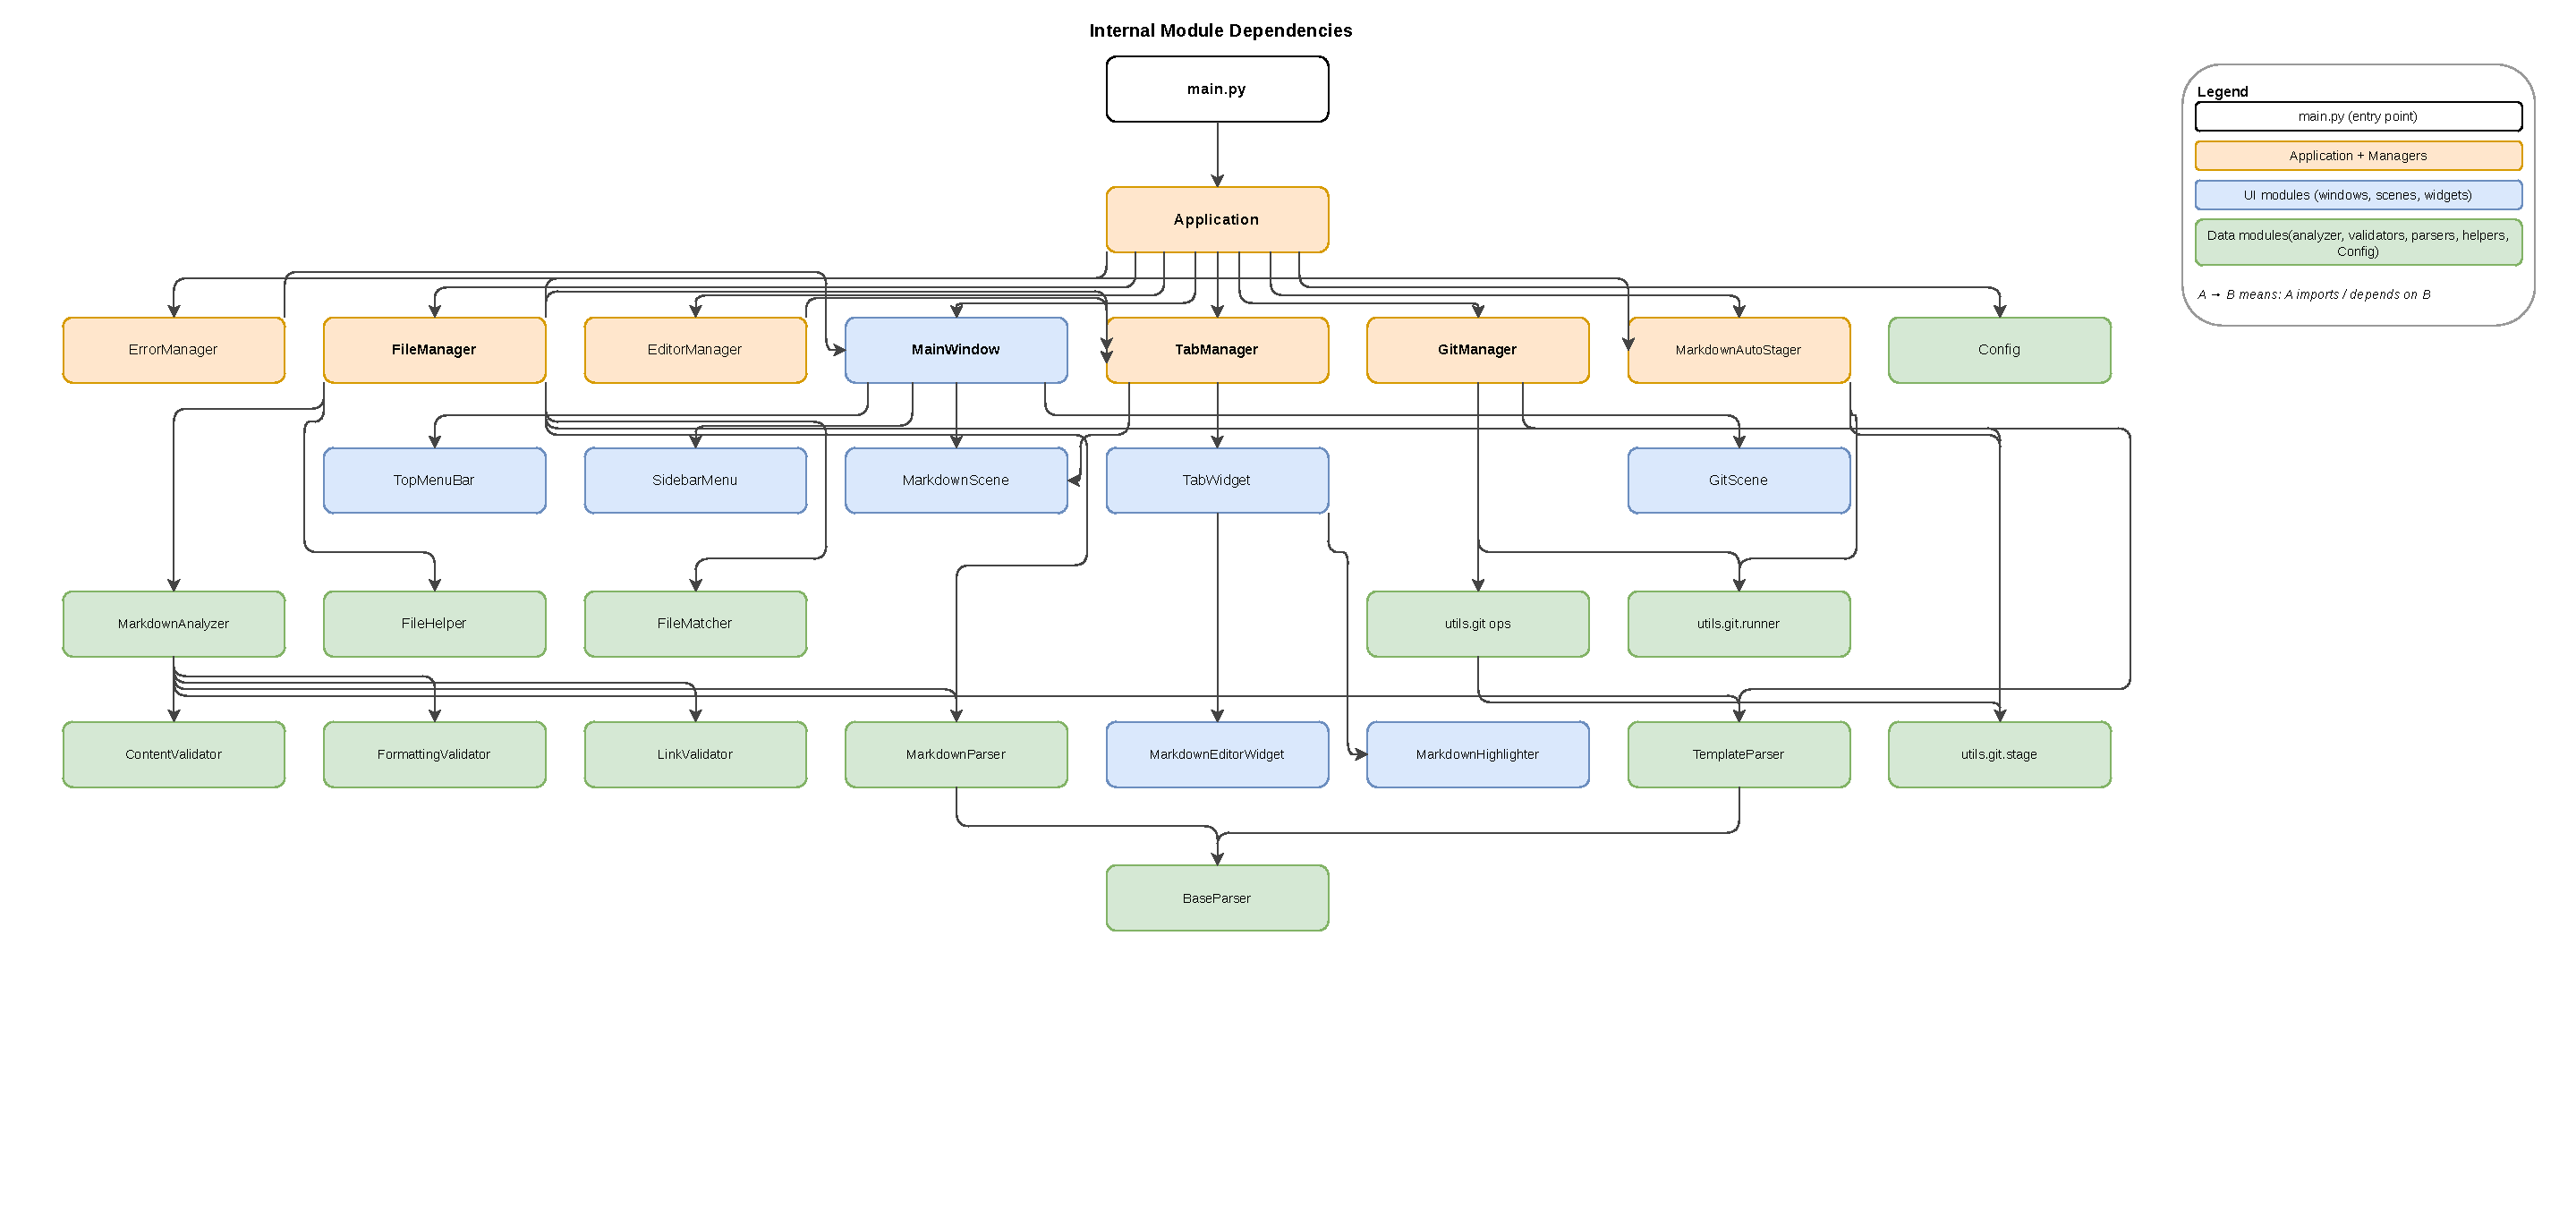
\includegraphics{images/dependency_diagram.pdf}}
    \caption{Závislosti hlavních modulů aplikace (importy a vrstvy mezi vstupním bodem, aplikací, manažery, uživatelským rozhraním a pomocnými knihovnami).}
    \label{fig:diagram-dependency}
\end{figure}

\subsubsection*{Tok dat při Git operacích}

Diagram \ref{fig:dataflow-git} popisuje dva paralelní toky. \textbf{Flow A} (vlevo)
reprezentuje uživatelem spouštěné Git operace (\emph{status}, \emph{fetch}, \emph{pull},
\emph{push}, \emph{export staged}): kliknutí v \texttt{GitScene} nebo v menu projde přes
\texttt{GitManager.start\_operation}, který vytvoří \texttt{GitOperationWorker}
(\texttt{QThread}) a v něm spustí příslušnou funkci z balíku \texttt{utils.git}
nad knihovnou GitPython. Výsledek (\texttt{GitResult}) se přes signály \texttt{operation\_output}
a \texttt{operation\_finished} vrací zpět do GUI vlákna a vypisuje se v konzoli \texttt{GitScene}.
\textbf{Flow B} (vpravo) ukazuje automatické stagování po uložení souboru: \texttt{FileManager}
vyvolá \texttt{MarkdownAutoStager.stage\_file\_delayed}, který přes jednorázový
\texttt{QTimer} (1\,s) spustí synchronní \texttt{stage\_markdown\_files} a o výsledku
informuje signály \texttt{file\_staged}\,/\,\texttt{staging\_failed}.

\begin{figure}[H]
    \centering
    \adjustbox{max width=\textwidth,max height=0.85\textheight,center}{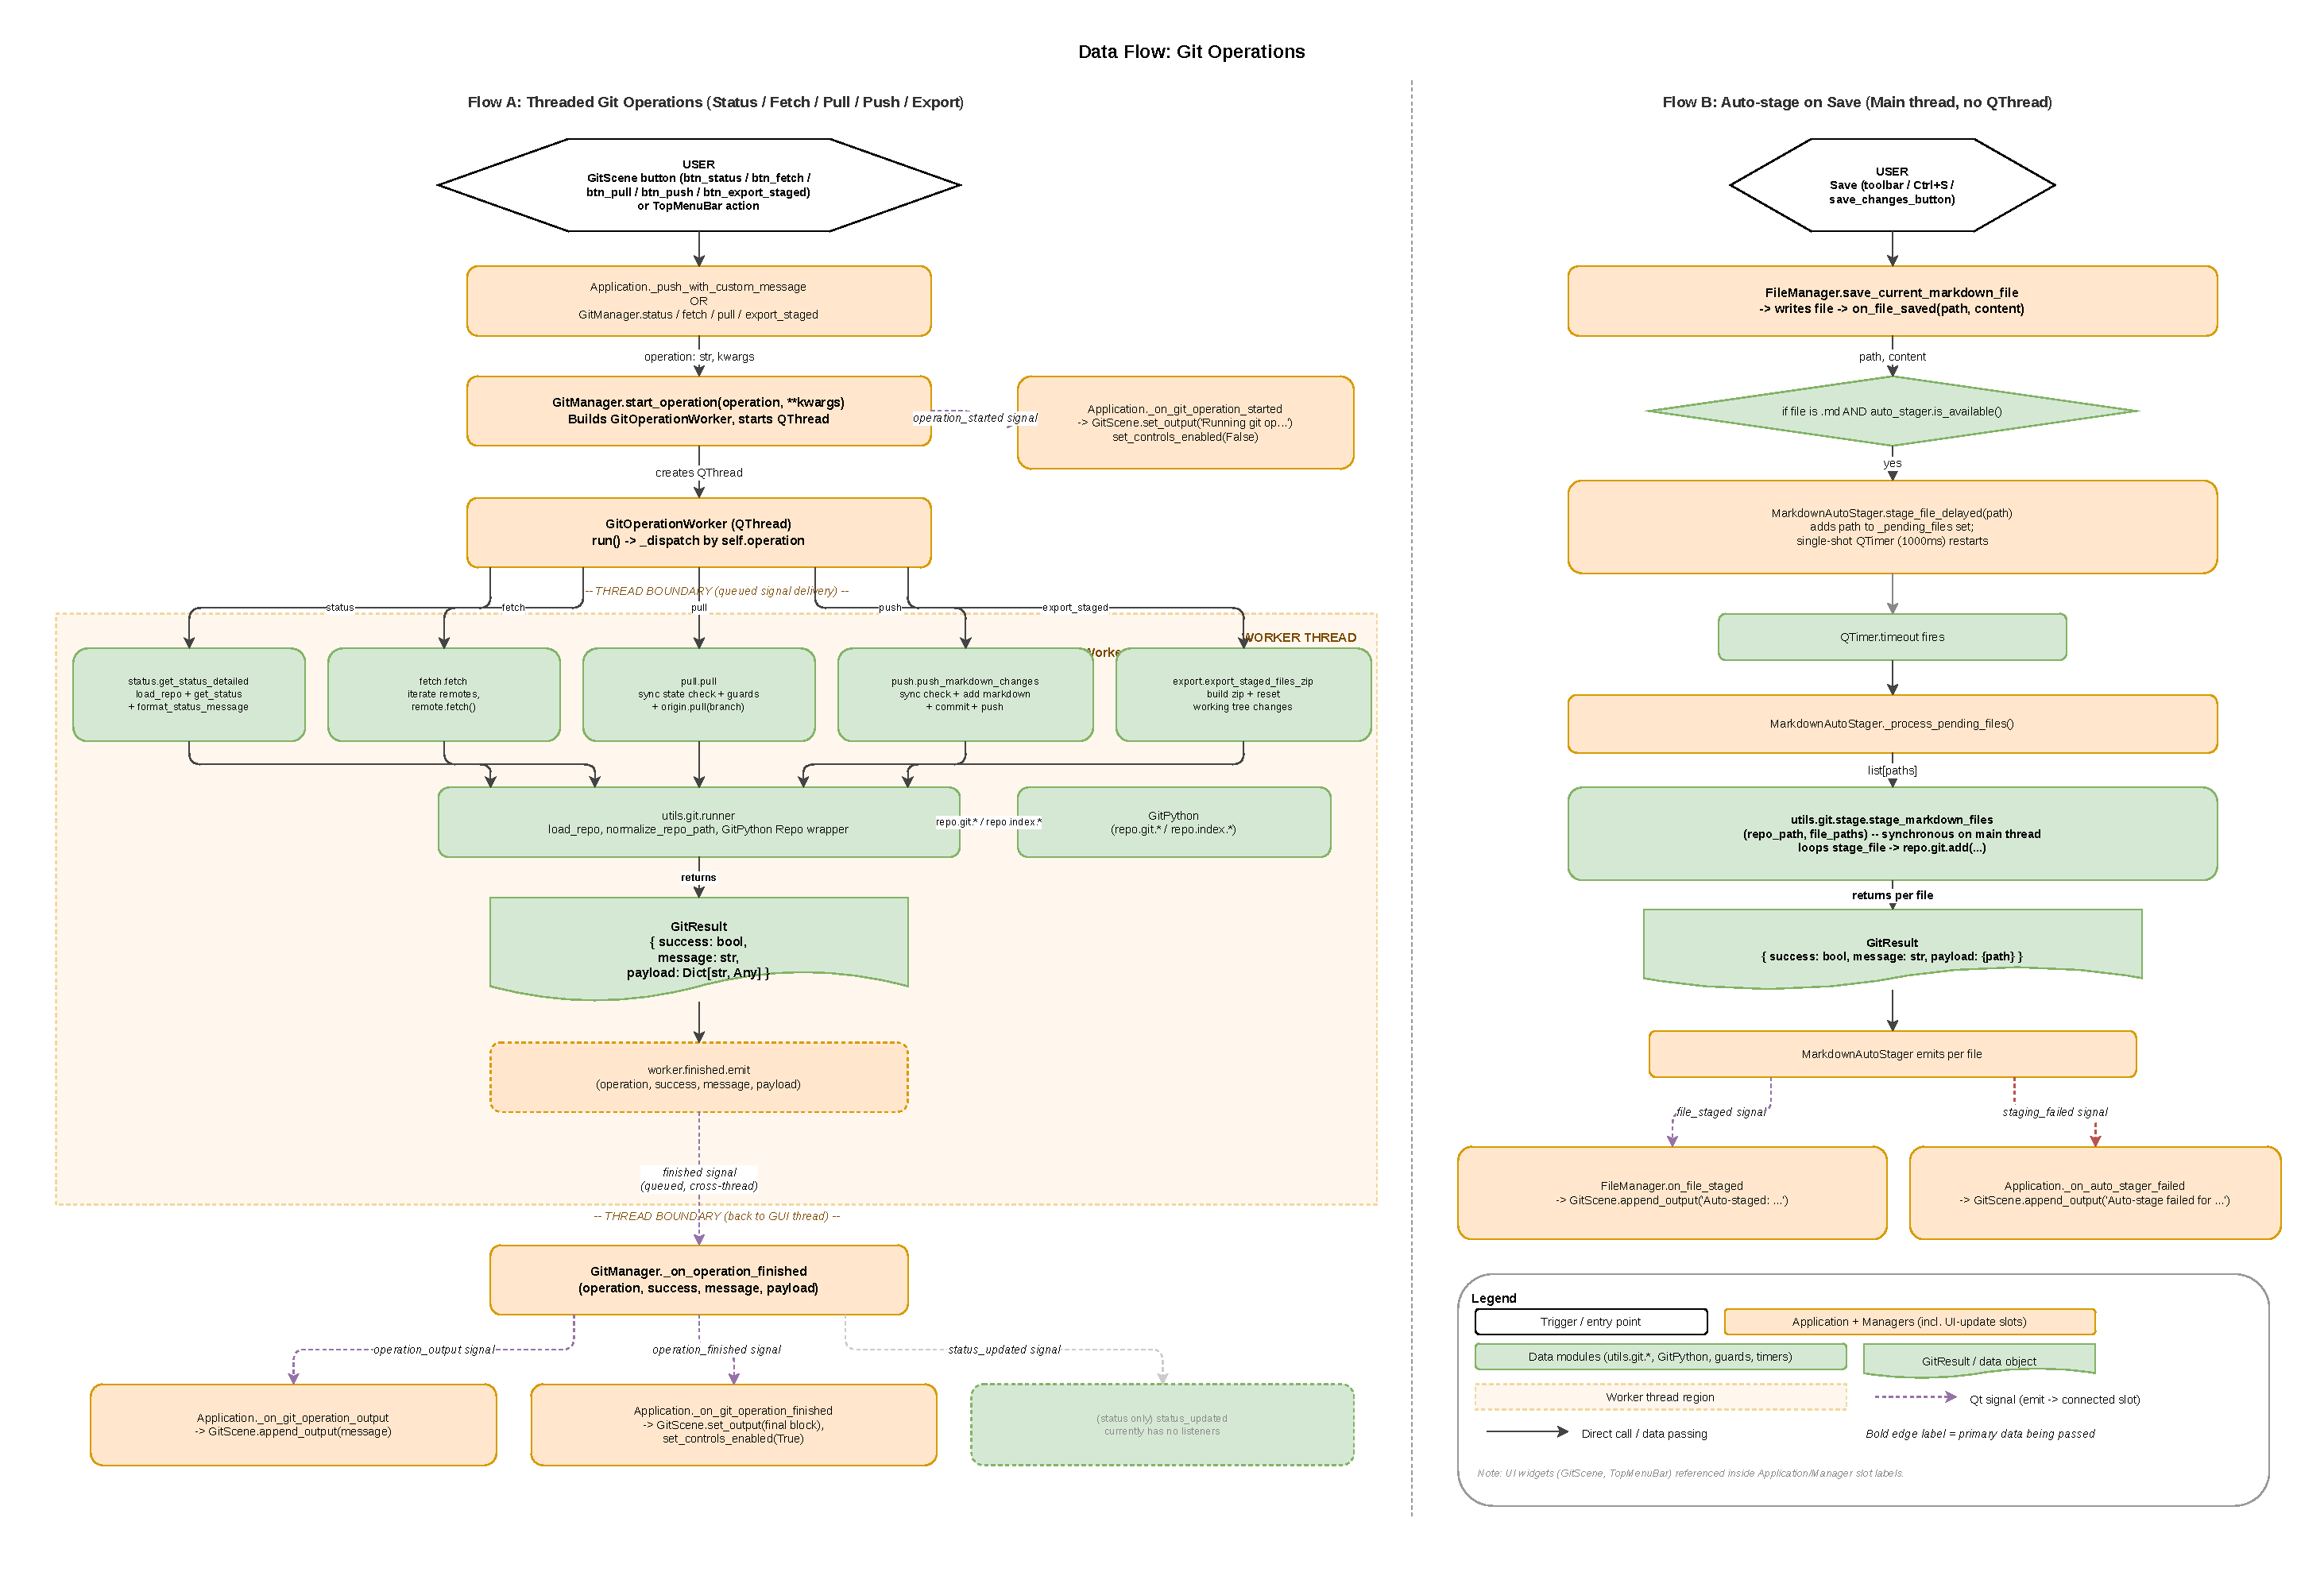
\includegraphics{images/dataflow_git.pdf}}
    \caption{Tok dat při Git operacích: akce uživatele v Git Scene nebo v menu, orchestrace v \texttt{GitManager}, provedení příkazů ve vlákně \texttt{GitOperationWorker} pomocí balíku \texttt{utils/git} a GitPython, zpětná vazba do konzole rozhraní.}
    \label{fig:dataflow-git}
\end{figure}

\subsubsection*{Tok dat při zobrazení markdown souboru}

Diagram \ref{fig:dataflow-display} ukazuje cestu od otevření souboru
(toolbar, dvojklik v průzkumníku, obnovení session nebo proklik v náhledu)
až do dvou souběžných pohledů. \texttt{FileManager.load\_markdown\_file} deleguje
validaci a načtení bytů na \texttt{FileHelper} (s detekcí kódování) a předá obsah
do \texttt{TabManager.load\_file\_into\_tab}. Z něj tečou data dvěma směry: do
\texttt{MarkdownEditorWidget} (kde \texttt{MarkdownHighlighter} provádí zvýraznění
syntaxe po blocích a vykresluje \emph{editor pane}) a -- přes signál \texttt{textChanged}
a \texttt{EditorManager.update\_live\_preview} -- do knihovny \texttt{markdown}
s rozšířeními \texttt{pymdownx}, jejíž HTML výstup je obalen výchozím CSS a zobrazen
v \texttt{QTextBrowser} jako \emph{preview pane}.

\begin{figure}[H]
    \centering
    \adjustbox{max width=\textwidth,max height=0.85\textheight,center}{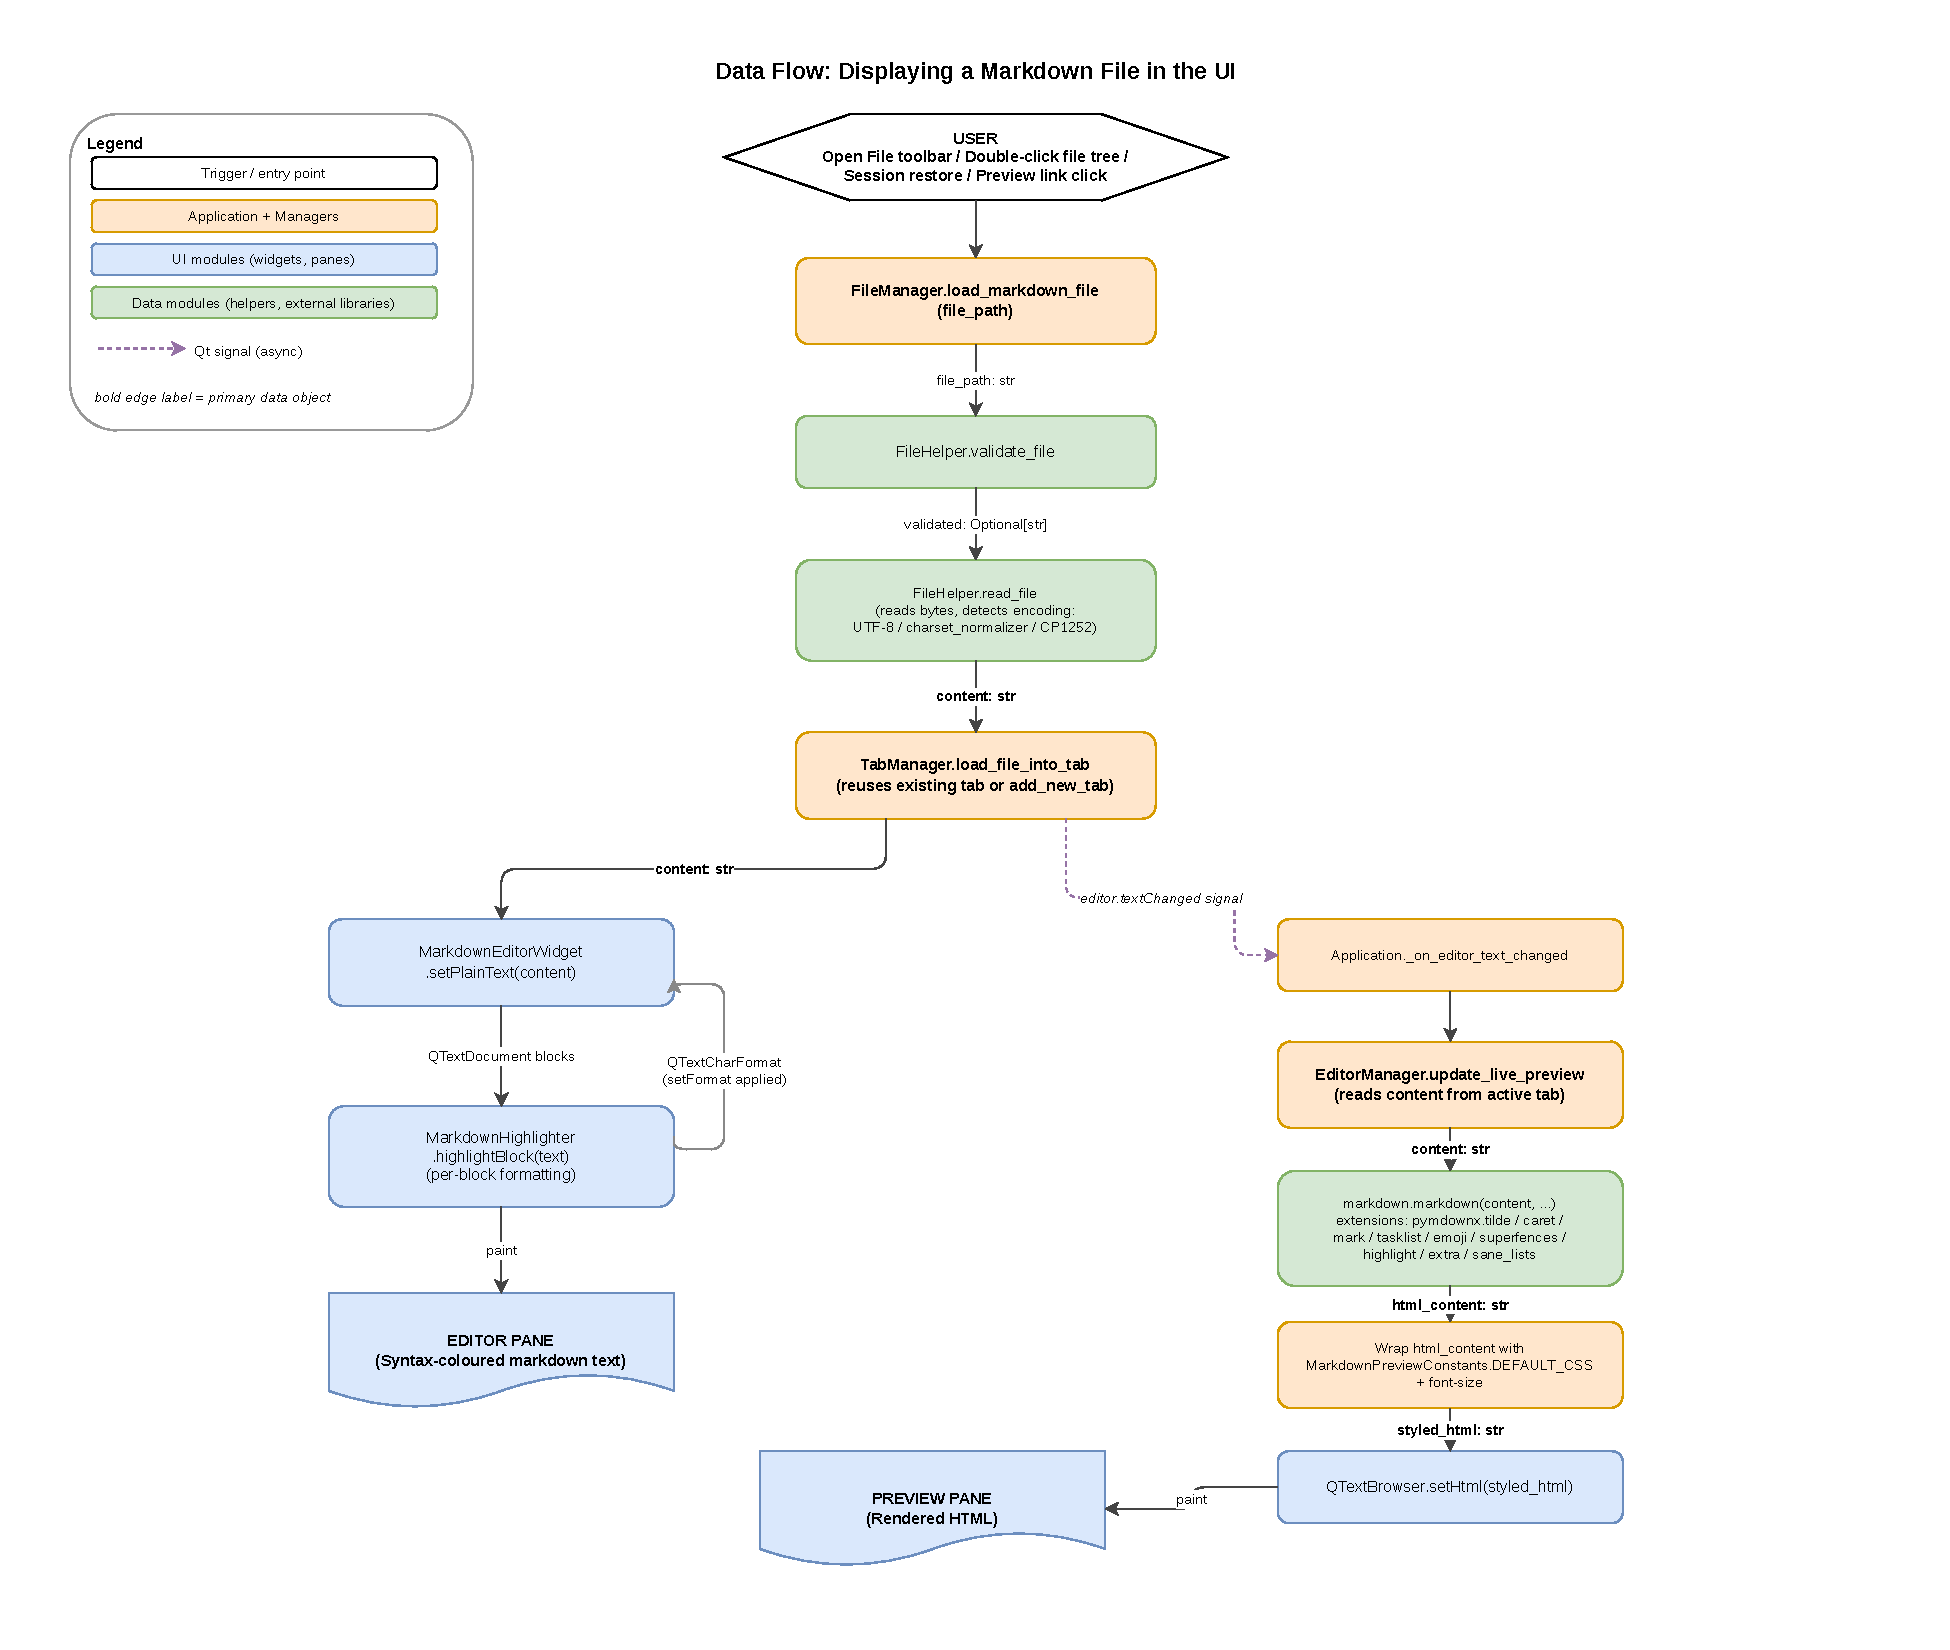
\includegraphics{images/dataflow_display.pdf}}
    \caption{Tok dat při zobrazení markdown souboru: \texttt{FileManager} využívá \texttt{FileHelper} k validaci a načtení obsahu, \texttt{TabManager} obsluhuje záložky a editor; živý náhled vzniká převodem markdownu na HTML a zobrazením v náhledovém widgetu.}
    \label{fig:dataflow-display}
\end{figure}

\subsubsection*{Tok dat při analýze a validaci}

Diagram \ref{fig:dataflow-analysis} ilustruje proces validace, který se spouští
po načtení nebo uložení markdown souboru. \texttt{FileManager.\_analyze\_current\_file}
paralelně získá dvě věci: \texttt{ParsedDocument} z \texttt{MarkdownParser.parse\_content}
a \texttt{TemplateRules} pro správnou šablonu, kterou \texttt{FileMatcher} dohledá
podle rodičovského adresáře souboru. Obě data putují do
\texttt{MarkdownAnalyzer.validate\_structure}, který spustí čtyři skupiny kontrol
(\texttt{FormattingValidator}, \texttt{ContentValidator}, vlastní kontroly H1
a sekcí, \texttt{LinkValidator}). Výsledný \texttt{analysis} dict
(\texttt{warnings} + \texttt{passed}) je převeden metodou \texttt{generate\_report}
na text a \texttt{TabManager.set\_analysis} ho po řádcích zobrazí v panelu
\texttt{analyzer\_list} jako barevně odlišené \texttt{QListWidgetItem} pod editorem
a náhledem.

\begin{figure}[H]
    \centering
    \adjustbox{max width=\textwidth,max height=0.85\textheight,center}{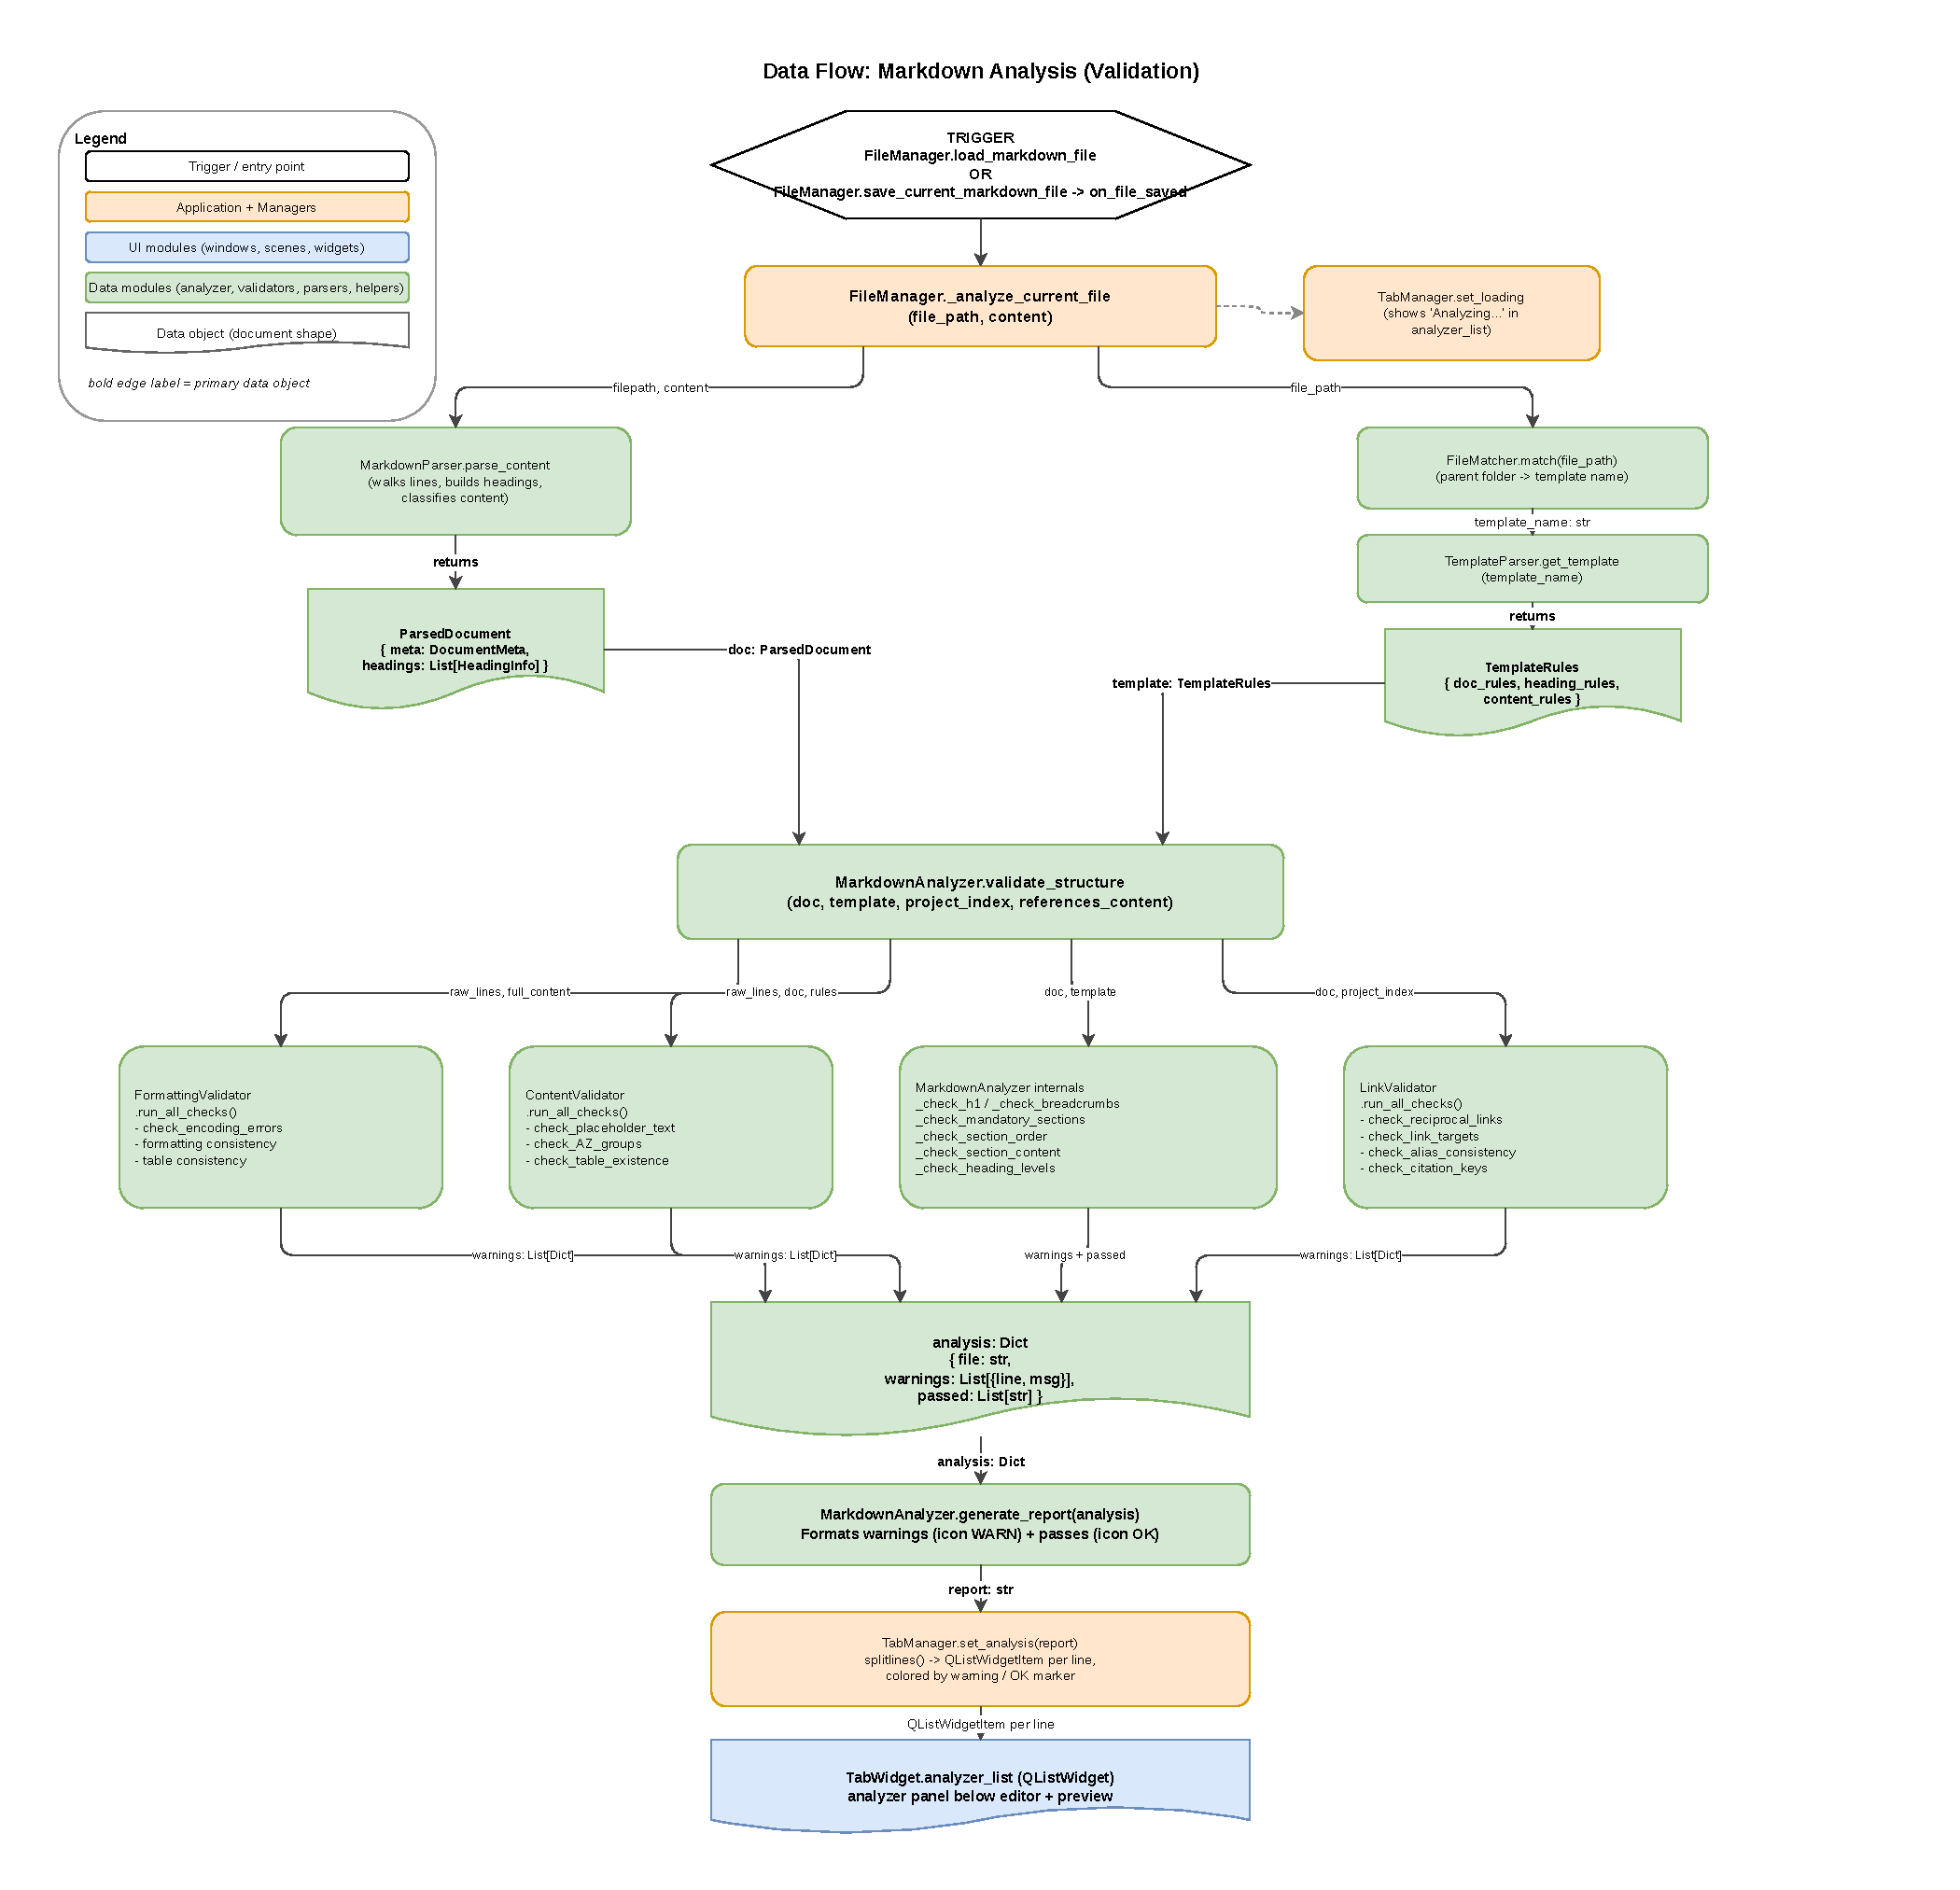
\includegraphics{images/dataflow_analysis.pdf}}
    \caption{Tok dat při analýze a validaci struktury markdownu po načtení nebo uložení: od \texttt{FileManager} přes parsování dokumentu, výběr šablony až po validátory a výpis výsledků v panelu analyzátoru.}
    \label{fig:dataflow-analysis}
\end{figure}

\subsection{Moduly}

Tato sekce popisuje logické a adresářové členění zdrojového kódu aplikace. Architektura projektu je navržena modulárně, 
s jasným oddělením uživatelského rozhraní (prezentační vrstvy) od aplikační logiky a pomocných nástrojů. 

\subsubsection{Core}

Modul \texttt{core} tvoří samotné jádro celé aplikace. Je zde soustředěna veškerá business logika, správa stavu, 
propojování komponent a analytické nástroje.

\begin{itemize}

    \item \textbf{\texttt{analyzer}} -- Tento balíček obsahuje veškerou logiku pro strukturální, obsahovou
    a formátovací kontrolu markdown souborů proti pravidlům šablon STePSEnHECs-PaCt. Vstupem analyzátoru
    je dvojice \texttt{ParsedDocument} (analyzovaný soubor) a \texttt{TemplateRules} (odpovídající šablona);
    výstupem je seznam varování (\texttt{warnings}) a úspěšně provedených kontrol (\texttt{passed}), které
    \texttt{TabManager} promítá do panelu Analyzer Output.

    \begin{itemize}
        \item \textbf{MarkdownAnalyzer} (\texttt{core/analyzer/markdown\_analyzer.py}):

        Hlavní orchestrátor analýzy. Postupně spouští všechny dílčí validátory
        (\texttt{FormattingValidator}, \texttt{ContentValidator}, \texttt{LinkValidator}) a sám provádí
        kontroly úrovně dokumentu: počet H1 nadpisů, shodu H1 se jménem souboru, shodu prefixu H1
        se šablonou, přítomnost a pořadí povinných sekcí, detekci sekcí, které šablona nezná, a kontrolu
        správné úrovně nadpisů. Dále validuje breadcrumb řádek dokumentu (počet částí, fixní hodnoty,
        existenci souborů odkazovaných z breadcrumbs). Pro speciální dokumenty
        (\texttt{template-publication}, in-memory šablony pro \emph{facets} a \emph{publications} indexy)
        vybrané kontroly přeskakuje. Výsledky umí převést do textového reportu
        metodou \texttt{generate\_report()}.

        \item \textbf{ContentValidator} (\texttt{core/analyzer/content\_validator.py}):

        Kontroluje obsah pod jednotlivými nadpisy. Ověřuje, že povinné sekce nejsou prázdné, že množina
        nalezených typů obsahu (\texttt{found\_types}) je nadmnožinou typů očekávaných šablonou
        (\texttt{expected\_types}), že hlavičky tabulek odpovídají šabloně, že bullet listy obsahují
        požadované prefixy (např.\ \texttt{(+)}, \texttt{(-)}) a že tabulka existuje tam, kde to šablona
        vyžaduje. U seskupených sekcí (A--Z bloky) porovnává množinu skutečně přítomných písmen s tou,
        kterou šablona definuje. Detekuje také kurzívní instrukce přebrané ze šablony
        (např.\ \emph{remove or replace this text}), které ve výsledném dokumentu nemají co dělat.

        \item \textbf{FormattingValidator} (\texttt{core/analyzer/formatting\_validator.py}):

        Soustředí kontroly nízkoúrovňového formátování textu. Hlídá liché počty hvězdiček
        (neuzavřený bold \texttt{**} nebo italic \texttt{*}, bullet markery jsou z řádku odfiltrovány),
        obrázky bez alt textu (\texttt{![](url)}), správnou skladbu tabulek a přítomnost
        Unicode \emph{replacement} znaku (\texttt{\textbackslash ufffd}), který indikuje
        poškozené kódování souboru.

        \item \textbf{LinkValidator} (\texttt{core/analyzer/links\_validator.py}):

        Validuje markdown odkazy na úrovni celého projektu pomocí globálního indexu souborů
        (\texttt{project\_index}). Ověřuje, že každý relativní odkaz na \texttt{.md} soubor existuje
        v projektu, že vzájemné odkazy mezi vzory v sekci \emph{Related Patterns} jsou reciproční
        (pokud vzor A odkazuje na vzor B, musí B odkazovat zpět na A) a že popisek odkazu odpovídá
        názvu cílového souboru nebo některému z jeho aliasů uvedených v sekci \emph{Also Known As}.
        Pro indexové šablony lze kontrolu aliasů přeskočit přepínačem \texttt{skip\_alias\_check}.
    \end{itemize}

    \item \textbf{\texttt{managers}} -- Tento balíček slouží jako hlavní řídicí (controller) vrstva aplikace. 
    Třídy v této složce oddělují aplikační logiku od samotného uživatelského rozhraní (UI). 
    Jejich úkolem je koordinace procesů, zpracování událostí z UI a komunikace mezi vizuálními 
    komponentami a nízkoúrovňovými nástroji (jako je analyzátor, Git nebo souborový systém).
    \begin{itemize}
        \item \textbf{EditorManager} (\texttt{core/managers/editor\_manager.py}):
        
        \texttt{EditorManager} má na starosti řízení samotného textového editoru a jeho doplňkových vizuálních panelů. 
        Zpracovává změny stavu přepínačů pro zobrazení živého náhledu a výstupu analyzátoru. Jeho klíčovou funkcí je 
        dynamické převádění surového markdownu do formátovaného HTML kódu pomocí knihovny \texttt{markdown} a 
        široké sady rozšíření \texttt{pymdownx}. Přebírá obsah z aktuální záložky (\texttt{TabManager}) a 
        zajišťuje jeho okamžitou vizuální reprezentaci v panelu \texttt{Live Preview}.

        \item \textbf{ErrorManager} (\texttt{core/managers/error\_manager.py}):

        \texttt{ErrorManager} centralizuje zobrazení vyskakovacích dialogů a chybových hlášení napříč celou aplikací. 
        Pomocí třídních (statických) metod poskytuje jednotné rozhraní pro vyvolání informačních zpráv, 
        varování, kritických chyb či interaktivních dotazů (jako je volba uložení/zahození změn při zavírání aplikace). 
        Všechna tato upozornění interně realizuje prostřednictvím standardní UI komponenty \texttt{QMessageBox}.

        \item \textbf{FileManager} (\texttt{core/managers/file\_manager.py}):

        \texttt{FileManager} koordinuje práci s dokumenty v uživatelském rozhraní: 
        načítání šablon z adresáře, otevírání a ukládání markdown souborů ve spolupráci se \texttt{TabManager}, 
        spouštění analýzy přes \texttt{MarkdownAnalyzer} a obsluhu průzkumníka souborů. Pro čtení, zápis a 
        dialogy deleguje na \texttt{FileHelper}. Propojení s oknem, menu a záložkami je navázáno z třídy 
        \texttt{Application} (\texttt{core/application.py}), včetně zpracování kliknutí na odkazy v náhledu.

        \item \textbf{GitManager} (\texttt{core/managers/git\_manager.py}):

        \texttt{GitManager} slouží jako správce pro operace s verzovacím systémem Git napojený na uživatelské rozhraní. 
        Aby nedocházelo k zamrzání aplikace při síťových nebo diskových operacích, 
        deleguje spouštění příkazů (např. \texttt{push}, \texttt{pull}, \texttt{commit}) na asynchronní pracovní vlákno 
        \texttt{GitOperationWorker}. O výsledcích, průběhu a chybách následně informuje UI pomocí systému událostí (signálů).

        \item \textbf{TabManager} (\texttt{core/managers/tab\_manager.py}):

        \texttt{TabManager} spravuje životní cyklus záložek v hlavním pracovním prostoru (\texttt{MarkdownScene}). 
        Pomocí pomocné datové třídy \texttt{TabState} udržuje kontext o každé otevřené záložce, včetně cesty 
        k načtenému souboru a indikace neuložených změn (tzv. \textit{dirty state}, reprezentovaný hvězdičkou v názvu). 
        Zajišťuje logiku otevírání, zavírání a přepínání záložek, předává textové změny k dalšímu zpracování a 
        rovněž propisuje formátované výsledky z analyzátoru do odpovídajícího UI panelu v konkrétní záložce.
    \end{itemize}

    \item \textbf{\texttt{application.py}} -- Třída \texttt{Application} představuje centrální bod celé aplikace. 
    Slouží k inicializaci všech klíčových komponent (hlavní okno, analyzátory, manažeři, pomocné nástroje) 
    a k propojení uživatelského rozhraní s aplikační logikou. Zajišťuje 
    propojení událostí z UI (jako jsou kliknutí na tlačítka, výběr z menu či změny zaškrtávacích políček) 
    s konkrétními akcemi v jednotlivých manažerech. Dále řídí životní cyklus aplikace, což zahrnuje 
    aplikaci grafického motivu (QSS), spuštění hlavní smyčky událostí, bezpečné načítání předchozího stavu 
    při startu (např. pozice okna, otevřené záložky, poslední adresář) a jeho ukládání při ukončování aplikace.

\end{itemize}

\subsubsection{Ui}

Modul \texttt{ui} obsahuje definici uživatelského rozhraní aplikace:

\begin{itemize}
    \item \textbf{\texttt{assets}} -- aktiva aplikace (ikony a \texttt{QSS} vzhledy.)
    \item \textbf{\texttt{components}} -- ui komponenty použité v jednotlivých scénách.
    \item \textbf{\texttt{scenes}} -- scény aplikace.
    \item \textbf{\texttt{main\_window.py}} -- definice hlavního okna apliakce.
\end{itemize}

\subsubsection{Utils}

Modul \texttt{utils} obsahuje pomocné nástroje apliakce.

\begin{itemize}
    \item FileHelper (\texttt{utils/file\_helper.py}):

    Třída \texttt{FileHelper} soustředí nízkoúrovňové operace se soubory a systémovými dialogy PyQt6. 
    Poskytuje výběr jednoho či více markdown souborů a pracovního adresáře (\texttt{QFileDialog}), 
    validaci existence souboru, typu a oprávnění ke čtení, čtení a zápis s detekcí kódování 
    (UTF-8, případně knihovna \texttt{charset\_normalizer}, záložní CP1252) a zapamatováním kódování pro konzistentní uložení. 
    Dále vyhledává markdown soubory v adresáři (s možností rekurze), hlídá rozumnou velikost obsahu podle \texttt{FileConstants} 
    a pomáhá při rozlišení relativních odkazů z náhledu (\texttt{resolve\_relative\_markdown\_link}).

    \item Git operace (\texttt{GitManager}, balík \texttt{utils/git}):

    Správu příkazů Git zajišťuje \texttt{GitManager} (\texttt{core/managers/git\_manager.py}),
    který ve vlastním vlákně spouští \texttt{GitOperationWorker} odvozený od \texttt{QThread}.
    V jeden okamžik může běžet nejvýše jedna operace; další požadavky jsou odmítnuty s hláškou pro uživatele.
    Pracovník podle typu operace volá funkce z balíku \texttt{utils/git}
    (stav repozitáře, fetch, pull, push včetně commit zprávy, staging, export staged změn do archivu apod.),
    přičemž práce s repozitářem probíhá přes knihovnu GitPython. Výsledky jsou předávány jako \texttt{GitResult}.
    Nebezpečná akce exportu vyžaduje potvrzení dialogem o možné ztrátě dat. Signály manažeru aktualizují Git Scene
    (konzole, povolení ovládacích prvků); konkrétní propojení je v \texttt{Application}.

    \item Parsery (balík \texttt{utils/parsers}):

    Balík \texttt{utils/parsers} převádí surový text markdown souborů a šablon na strukturované
    datové třídy, se kterými následně pracuje analyzátor. Aby se logika rozpoznávání nadpisů,
    breadcrumbs a typů obsahu neopakovala ve dvou modulech, je veškerá regexová a klasifikační
    logika soustředěna do sdíleného modulu \texttt{base\_parser}.

    \begin{itemize}
        \item \textbf{base\_parser} (\texttt{utils/parsers/base\_parser.py}):

        Modul sdílených parsovacích primitiv. Obsahuje funkce \texttt{parse\_heading\_line()}
        (rozparsuje řádek nadpisu na úroveň, čistý text, odkaz a u šablon i indikátory \emph{optional}
        a italických \emph{variable} placeholderů), \texttt{split\_h1()} (rozdělí H1 na prefix a hodnotu
        podle dvojtečky), \texttt{parse\_breadcrumbs()} (rozpozná breadcrumb řádek od italic instrukcí
        šablony) a \texttt{classify\_content\_line()} (klasifikuje řádek obsahu na typy text, bullet
        list, tabulka, obrázek, odkaz, horizontální čára nebo footnote a extrahuje hlavičky tabulky
        a bullet prefixy). Všechny ostatní parsery pracují právě nad těmito funkcemi.

        \item \textbf{MarkdownParser} (\texttt{utils/parsers/markdown\_parser.py}):

        Převádí načtený markdown soubor na \texttt{ParsedDocument}. Výstupem je dvojice
        \texttt{DocumentMeta} (cesta k souboru, breadcrumbs v originálním i normalizovaném tvaru,
        prefix a hodnota H1) a seznam \texttt{HeadingInfo} (úroveň nadpisu, text, číslo řádku
        a vnořené \texttt{ContentInfo} s nalezenými typy obsahu, bullet prefixy, hlavičkami tabulky
        a tzv.\ \emph{raw\_lines} pro pozdější kontroly formátování). Souvislé běhy A--Z nadpisů
        jsou automaticky sbaleny do jediného \texttt{is\_group=True} záznamu, aby je bylo možné
        porovnávat se šablonou jako celek. Metoda \texttt{get\_link\_metadata()} navíc z dokumentu
        vytáhne aliasy (sekce \emph{Also Known As}) a vzájemné odkazy (\emph{Related Patterns});
        výsledky se promítají do globálního \texttt{project\_index}, nad kterým pracuje
        \texttt{LinkValidator}.

        \item \textbf{TemplateParser} (\texttt{utils/parsers/template\_parser.py}):

        Analogie \texttt{MarkdownParser} pro šablonové soubory. Výstupem je \texttt{TemplateRules}
        obsahující \texttt{DocumentRules} (očekávané breadcrumbs, prefix H1) a seznam
        \texttt{HeadingRules} s vnořenými \texttt{ContentRules} (očekávané typy obsahu, povinné bullet
        prefixy, hlavičky tabulek). Parser navíc detekuje markery \emph{(optional)} a italické
        \emph{variable} placeholdery v nadpisech a stejně jako dokumentový parser sbaluje A--Z bloky.
        Načtené šablony jsou udržovány v interní mapě \texttt{templates} a vyhledávány podle jména.

        \item \textbf{FileMatcher} (\texttt{utils/file\_matcher.py}):

        Páruje konkrétní markdown soubor s odpovídající šablonou na základě jména rodičovského
        adresáře (např.\ soubory v adresáři \texttt{patterns/} se validují proti šabloně
        \texttt{template-pattern}). Speciální případy jako indexy \emph{facets} a publikační
        soubory jsou ošetřeny pomocí in-memory šablon z modulu \texttt{facets\_index\_template}.

        \item \textbf{facets\_index\_template} (\texttt{utils/facets\_index\_template.py}):

        Definuje \texttt{TemplateRules} programaticky, bez načítání ze souboru, pro dokumenty,
        které nemají odpovídající \texttt{.md} šablonu na disku
        (indexy podle facet, seznam publikací). Tyto šablony mají volnější pravidla --
        povolují variabilní H1 a libovolný textový obsah.

        \item \textbf{Konstanty a výjimky} (\texttt{utils/constants.py}, \texttt{utils/exceptions.py}):

        Soubor \texttt{constants.py} centralizuje všechny tzv.\ magické hodnoty -- regulární výrazy
        pro nadpisy, odkazy a breadcrumbs, povolené přípony souborů, limity velikosti, ikony pro
        report (\texttt{ICON\_OK}, \texttt{ICON\_WARNING}) i konstanty pro Git operace.
        Soubor \texttt{exceptions.py} definuje hierarchii vlastních výjimek
        (\texttt{BaseAppException}, \texttt{GitException}, \texttt{FileNotFoundError},
        \texttt{InvalidInputError}, \ldots) s podporou uživatelsky srozumitelných hlášek a titulků
        dialogů, díky čemuž \texttt{ErrorManager} dokáže zobrazit konzistentní chybové zprávy.
    \end{itemize}
\end{itemize}

\section{Validace markdown souborů}

Validace markdown souborů je hlavní funkcí aplikace. Cílem je ověřit, že každý dokument
katalogu STePSEnHECs-PaCt odpovídá pravidlům příslušné šablony -- má správně sestavený
nadpis, breadcrumbs, sekce v očekávaném pořadí, smysluplný obsah pod každou sekcí a funkční
vzájemné odkazy mezi vzory. Tok dat při validaci je znázorněn na obrázku
\ref{fig:dataflow-analysis}.

\subsection{Princip validace}

Postup validace je rozdělen do tří kroků:

\begin{enumerate}
    \item \textbf{Parsování dokumentu a šablony.} \texttt{MarkdownParser} převede obsah souboru
    na \texttt{ParsedDocument} (metadata, seznam nadpisů a strukturovaný obsah pod každým z nich).
    \texttt{TemplateParser} převede odpovídající šablonu na \texttt{TemplateRules}.
    Spárování dokumentu se šablonou zajišťuje \texttt{FileMatcher} na základě jména rodičovského
    adresáře (např.\ \texttt{patterns/} $\rightarrow$ \texttt{template-pattern}); pro indexové soubory
    se použijí in-memory šablony z modulu \texttt{facets\_index\_template}.

    \item \textbf{Spuštění dílčích validátorů.} \texttt{MarkdownAnalyzer} jako orchestrátor postupně
    spustí \texttt{FormattingValidator} (formátování textu), \texttt{ContentValidator}
    (obsah jednotlivých sekcí), kontroly struktury a breadcrumbs ve vlastním těle a nakonec
    \texttt{LinkValidator} (vzájemné odkazy v rámci celého projektu, pokud je k dispozici globální
    \texttt{project\_index}). Každý validátor pracuje nad společnými datovými třídami a vrací dva
    seznamy: \texttt{warnings} (nalezené chyby) a \texttt{passed} (úspěšně splněné kontroly).

    \item \textbf{Agregace a zobrazení výsledků.} Výsledky všech validátorů jsou sloučeny,
    seřazeny podle čísla řádku a předány \texttt{TabManager}, který je zobrazí v panelu
    Analyzer Output s barevným odlišením úspěchů, varování a chyb.
\end{enumerate}

\subsection{Přehled validačních pravidel}

Následující tabulka shrnuje všechna kontrolovaná pravidla, sloupec \emph{Kde se implementuje}
odkazuje na umístění kontroly v kódu: \texttt{document\_loader} = během parsování v
\texttt{MarkdownParser}, \emph{validátor} = některý z validátorů v balíku
\texttt{core/analyzer}, \emph{oboje} = pravidlo je z části detekováno už při parsování
(uložení potřebných dat do \texttt{ParsedDocument}) a finálně vyhodnoceno validátorem.

\renewcommand{\arraystretch}{1.25}
\begin{small}
\begin{longtable}{|c|p{3.0cm}|p{8.5cm}|p{2.5cm}|}
\hline
\textbf{\#} & \textbf{Kategorie} & \textbf{Co se ověřuje} & \textbf{Kde se implementuje} \\
\hline
\endfirsthead
\hline
\textbf{\#} & \textbf{Kategorie} & \textbf{Co se ověřuje} & \textbf{Kde se implementuje} \\
\hline
\endhead

1 & Struktura dokumentu & Dokument musí mít právě jeden H1 nadpis. & document\_loader \\ \hline
2 & Struktura dokumentu & \texttt{dokument.h1\_value} (case-insensitive) == stem souboru. & document\_loader \\ \hline
3 & Struktura dokumentu & Prefix v H1 musí souhlasit s tím, co šablona definuje. & oboje \\ \hline
4 & Struktura dokumentu & Všechny non-optional headingy ze šablony musí existovat v dokumentu. & oboje \\ \hline
5 & Struktura dokumentu & Pokud optional sekce existuje, její text musí odpovídat šabloně. & oboje \\ \hline
6 & Struktura dokumentu & Sekce musí být ve stejném pořadí jako v šabloně. & oboje \\ \hline
7 & Struktura dokumentu & Dokument neobsahuje headingy, které šablona vůbec nezná. & oboje \\ \hline
8 & Struktura dokumentu & Sekce musí mít správnou úroveň (\#, \#\#, \#\#\#\ldots) podle šablony. & oboje \\ \hline
9 & Breadcrumbs & Dokument musí mít breadcrumb řádek. & document\_loader \\ \hline
10 & Breadcrumbs & Počet částí oddělených '>' musí odpovídat šabloně. & oboje \\ \hline
11 & Breadcrumbs & Fixní části (ne poslední) musí textově odpovídat šabloně. & oboje \\ \hline
12 & Breadcrumbs & Každý \texttt{[label](url)} v breadcrumbs odkazuje na existující soubor. & validátor \\ \hline
13 & Obsah sekcí & Non-optional sekce musí mít alespoň nějaký obsah. & oboje \\ \hline
14 & Obsah sekcí & \texttt{found\_types} musí být nadmnožinou \texttt{expected\_types} (kromě 'text'). & oboje \\ \hline
15 & Obsah sekcí & Sloupce tabulky musí odpovídat šabloně. & oboje \\ \hline
16 & Obsah sekcí & Pokud šablona definuje \texttt{bullet\_prefixes}, dokument je musí obsahovat. & oboje \\ \hline
17 & Obsah sekcí & V dokumentu nesmí zůstat kurzívní instrukce ze šablony (např.\ 'remove or replace\ldots'). & oboje \\ \hline
18 & Obsah sekcí & Dokument musí mít kompletní sadu písmen dle šablony. & oboje \\ \hline
19 & Obsah sekcí & Tabulka existuje, ale může být prázdná. & oboje \\ \hline
20 & Formátování & Liché počty \texttt{**} na řádku = neuzavřený bold. & oboje \\ \hline
21 & Formátování & Liché počty \texttt{*} (mimo bullet marker) = neuzavřená italic. & oboje \\ \hline
22 & Formátování & \texttt{![](url)} bez alt textu = přístupnostní chyba. & oboje \\ \hline
23 & Formátování & Přítomnost replacement character ($\square$, \texttt{\textbackslash ufffd}) = špatné kódování souboru. & oboje \\ \hline
24 & Formátování & Správně zadaná tabulka. & oboje \\ \hline
25 & Linky & \texttt{[](url)} nebo \texttt{[label]()} = špatně zadaný odkaz. & document\_loader \\ \hline
26 & Linky & \texttt{[label](relativní\_cesta)} musí odkazovat na existující soubor. & document\_loader \\ \hline
27 & Linky & Pokud pattern A odkazuje v sekci 'Related Patterns' na pattern B, pak B musí mít odkaz zpět na A. & validátor \\ \hline
28 & Linky & Pokud je v A--Z sekci odkaz na pattern pod jiným názvem (alias), ověřit, že cílový soubor existuje a cílový pattern má alias v sekci 'Also Known As'. & validátor \\ \hline

\caption{Přehled validačních pravidel aplikovaných na markdown soubory.}
\label{tab:validation-rules}
\end{longtable}
\end{small}
\renewcommand{\arraystretch}{1.0}

\section{Uživatelské rozhraní}

Aplikace plně využívá vlastní tmavý motiv (Dark Mode) a vektorové ikony. 
Rozhraní je rozděleno do dvou hlavních pracovních pohledů (scén), mezi kterými lze přepínat.

\subsection{Hlavní rozvržení okna}
\begin{itemize}
    \item \textbf{Postranní panel (Sidebar):} Úzký svislý panel na levé straně okna, který slouží k rychlému přepínání mezi editorem Markdownu a rozhraním pro správu Gitu.
    \item \textbf{Horní menu a lišta (Toolbar):} Poskytuje přístup k nejpoužívanějším akcím (otevírání souborů a složek, ukládání, spouštění Git operací) a obsahuje klávesové zkratky.
\end{itemize}

\subsection{Pracovní pohled Markdown (Markdown Scene)}
Tento pohled je primárním rozhraním pro úpravu a analýzu markdown souborů.
\begin{itemize}
    \item \textbf{Průzkumník souborů (File Explorer):} Levý postranní panel zobrazující stromovou strukturu načteného pracovního adresáře. Umožňuje rychlou navigaci a otevírání dokumentů dvojitým kliknutím. Pro maximalizaci pracovního prostoru lze panel skrýt.
    \item \textbf{Správce záložek (Tab Manager):} Centrální pracovní plocha umožňující editaci více souborů současně. Záložky vizuálně indikují neuložené změny (hvězdičkou) a chrání uživatele před ztrátou dat při zavření okna.
    \item \textbf{Ovládací panel editoru:} Obsahuje rychlé přepínače (checkboxy) pro zobrazení nebo skrytí živého náhledu a výstupu analyzátoru.
    \item \textbf{Živý náhled (Live Preview):} Panel umístěný napravo od textového editoru, který v reálném čase vykresluje formátovaný HTML výstup (včetně syntaxe kódu, tabulek a odkazů) na základě psaného textu.
    \item \textbf{Výstup analyzátoru (Analyzer Output):} Spodní panel v rámci záložky, který interaktivně vypisuje výsledky strukturální kontroly a validace odkazů. Barvami (červená/žlutá/zelená) odlišuje úspěšné kontroly, varování a kritické chyby.
\end{itemize}

\subsection{Pracovní pohled Git (Git Scene)}
Tento pohled slouží k integraci s verzovacím systémem a poskytuje grafické rozhraní pro správu repozitáře.
\begin{itemize}
    \item \textbf{Vstupní pole pro zprávu:} Víceřádkové textové pole, které vynucuje zadání zprávy ke commitu před odesláním změn.
    \item \textbf{Ovládací panel Gitu:} Tlačítka pro spouštění asynchronních git operací (\texttt{Status}, \texttt{Fetch}, \texttt{Pull}, \texttt{Push}, \texttt{Export Staged}).
    \item \textbf{Konzole (Output Console):} Textový výpis umístěný uprostřed, který uživateli poskytuje přímou zpětnou vazbu o probíhajících Git operacích a loguje automatické přidávání souborů (auto-staging) běžící na pozadí.
\end{itemize}

\section{Testování}

\subsection{Jednotkové testy}

Jednotkové testy aplikace jsou napsané v frameworku \texttt{pytest} a leží v adresáři
\texttt{application/tests/}. Testy jsou tematicky rozděleny do podadresářů
\texttt{analyzers/}, \texttt{parsers/}, \texttt{file/} a \texttt{git/}, které kopírují
strukturu produkčního kódu. Sdílené fixtures (např.\ inicializace prázdného Git repozitáře
s počátečním commitem) jsou definovány v \texttt{conftest.py} a \texttt{tests/fixtures/}.

Testy se spouští z adresáře \texttt{application/} příkazem \texttt{pytest tests/} (případně
s přepínači \texttt{-v} pro podrobný výpis nebo \texttt{--cov=core --cov=utils} pro měření
pokrytí). Každý test je nezávislý -- využívá pytest fixtures \texttt{tmp\_path}
pro dočasné soubory, takže testy nezasahují do skutečného souborového systému ani Git repozitáře
projektu.

\subsubsection*{Testy analyzátoru (\texttt{tests/analyzers/})}

\begin{itemize}
    \item \textbf{\texttt{test\_markdown\_analyzer.py}} -- pokrývá orchestrátor
    \texttt{MarkdownAnalyzer}: inicializaci s vlastním i výchozím \texttt{base\_path},
    kontroly počtu H1 nadpisů, shody H1 se jménem souboru, prefixu H1, povinných sekcí,
    pořadí sekcí, detekce neznámých sekcí, úrovní nadpisů, validace breadcrumbs a jejich
    odkazů, vyhledávání markdown odkazů a generování textového reportu.

    \item \textbf{\texttt{test\_content\_validator.py}} -- pokrývá kontroly obsahu sekcí:
    prázdné povinné sekce, shodu \texttt{found\_types} s \texttt{expected\_types},
    sloupce a existenci tabulek, povinné bullet prefixy, detekci kurzívních instrukcí
    přebraných ze šablony a kontroly úplnosti A--Z bloků.

    \item \textbf{\texttt{test\_formatting\_validator.py}} -- pokrývá nízkoúrovňové kontroly
    formátování: neuzavřený bold a italic, obrázky bez alt textu, korektnost tabulek
    a detekci Unicode \emph{replacement} znaku.

    \item \textbf{\texttt{test\_links\_validator.py}} a \textbf{\texttt{test\_relative\_checking.py}} --
    pokrývají \texttt{LinkValidator}: kontrolu existence cílů relativních odkazů,
    reciproční odkazy mezi vzory v sekci \emph{Related Patterns} a konzistenci aliasů
    se sekcí \emph{Also Known As}.
\end{itemize}

\subsubsection*{Testy parserů (\texttt{tests/parsers/})}

\begin{itemize}
    \item \textbf{\texttt{test\_base\_parser.py}} -- pokrývá sdílené parsovací primitivy:
    \texttt{parse\_heading\_line()} (úrovně nadpisů, optional a variable markery,
    odkazy v nadpisech), \texttt{split\_h1()}, \texttt{parse\_breadcrumbs()}
    (rozlišení od italic instrukcí) a \texttt{classify\_content\_line()} pro všechny
    typy obsahu (text, bullet, tabulka, obrázek, odkaz, footnote, horizontal rule).

    \item \textbf{\texttt{test\_markdown\_parser.py}} -- pokrývá \texttt{MarkdownParser}:
    sestavení \texttt{ParsedDocument} z různých vstupů, korektní vyplnění
    \texttt{DocumentMeta} (breadcrumbs, prefix a hodnota H1), sbalení A--Z bloků
    do skupinových nadpisů a extrakci aliasů a vzájemných odkazů metodou
    \texttt{get\_link\_metadata()}.

    \item \textbf{\texttt{test\_template\_parser.py}} -- pokrývá \texttt{TemplateParser}:
    rozpoznání povinných a optional sekcí, italických \emph{variable} placeholderů,
    pravidel obsahu (\texttt{ContentRules}), správné sestavení \texttt{HeadingRules}
    a sbalení A--Z bloků v šabloně.
\end{itemize}

\subsection{Testovací scénáře}

Tato sekce obsahuje hlavní funkční testy pro aplikaci, se zaměřením na uživatelské rozhraní, ošetření chyb a integraci Gitu.

\subsection*{1. Operace s Gitem (Git Operations)}

Scénář 1.1: Provedení Git Push se zadanou commit zprávou:

\textbf{Popis:} Ověření, že aplikace provede push, pokud uživatel zadá zprávu ke commitu.
\begin{itemize}
    \item \textbf{DÁNO} uživatel se nachází v pohledu Git (Git scene) a má připravené (staged) změny.
    \item \textbf{A} textové pole pro commit zprávu obsahuje text.
    \item \textbf{KDYŽ} uživatel klikne na tlačítko "Push".
    \item \textbf{PAK} operace Git push na pozadí se PROVEDE.
\end{itemize}

Scénář 1.2: Zamezení Git Push s prázdnou commit zprávou:

\textbf{Popis:} Ověření, že aplikace zablokuje push, pokud uživatel zapomene zadat zprávu ke commitu.
\begin{itemize}
    \item \textbf{DÁNO} uživatel se nachází v pohledu Git (Git scene) a má připravené (staged) změny.
    \item \textbf{A} textové pole pro commit zprávu je zcela prázdné (nebo obsahuje jen mezery).
    \item \textbf{KDYŽ} uživatel klikne na tlačítko "Push".
    \item \textbf{PAK} se zobrazí kritický dialog s titulkem "Missing Commit Message".
    \item \textbf{A} operace Git push na pozadí se NEPROVEDE.
\end{itemize}

Scénář 1.3: Export změněných souborů:

\textbf{Popis:} Ověření, že uživatel úspěšně exportuje změněné soubory z pracovního adresáře.
\begin{itemize}
    \item \textbf{DÁNO} uživatel se nachází v pohledu Git.
    \item \textbf{KDYŽ} uživatel klikne na tlačítko "Export Staged".
    \item \textbf{PAK} se zobrazí varovný dialog s titulkem "Warning: Potential Data Loss".
    \item \textbf{KDYŽ} uživatel klikne na "Ano" (Yes).
    \item \textbf{PAK} se dialog zavře a operace exportu se provede.
\end{itemize}

Scénář 1.4: Zamezení nechtěné ztrátě dat při Git Exportu:

\textbf{Popis:} Ověření, že je uživatel varován před exportem, protože tato akce vyčistí pracovní adresář.
\begin{itemize}
    \item \textbf{DÁNO} uživatel se nachází v pohledu Git.
    \item \textbf{KDYŽ} uživatel klikne na tlačítko "Export Staged".
    \item \textbf{PAK} se zobrazí varovný dialog s titulkem "Warning: Potential Data Loss".
    \item \textbf{KDYŽ} uživatel klikne na "Ne" (No).
    \item \textbf{PAK} se dialog zavře a operace exportu se zruší.
\end{itemize}

\subsection*{2. Ukončení aplikace a správa záložek (Tab Management)}

Scénář 2.1: Zavírání aplikace s neuloženými záložkami (Cancel):

\textbf{Popis:} Ověření, že uživatel může přerušit zavírání aplikace, pokud má neuloženou práci.
\begin{itemize}
    \item \textbf{DÁNO} aplikace je otevřená a obsahuje alespoň jednu neuloženou záložku (indikováno hvězdičkou * v názvu záložky).
    \item \textbf{KDYŽ} uživatel klikne na systémové tlačítko pro zavření okna ('X').
    \item \textbf{PAK} se zobrazí varovný dialog s dotazem na Uložení (Save), Zahození (Discard) nebo Zrušení (Cancel).
    \item \textbf{KDYŽ} uživatel klikne na "Cancel".
    \item \textbf{PAK} se dialog zavře a aplikace zůstane otevřená.
\end{itemize}

Scénář 2.2: Uložení neuložených záložek při zavírání aplikace:

\textbf{Popis:} Ověření, že uživatel může úspěšně uložit svou práci během procesu ukončování aplikace.
\begin{itemize}
    \item \textbf{DÁNO} aplikace je otevřená s neuloženou záložkou.
    \item \textbf{KDYŽ} uživatel klikne na systémové tlačítko pro zavření okna ('X').
    \item \textbf{A} zobrazí se varovný dialog s dotazem na Uložení (Save), Zahození (Discard) nebo Zrušení (Cancel).
    \item \textbf{KDYŽ} uživatel klikne na "Save".
    \item \textbf{PAK} Uloží se daný soubor.
    \item \textbf{A} aplikace se ukončí.
\end{itemize}

Scénář 2.3: Zahození změn při zavírání aplikace:

\textbf{Popis:} Ověření, že uživatel může úmyslně zahodit změny a vynutit zavření aplikace.
\begin{itemize}
    \item \textbf{DÁNO} aplikace je otevřená s neuloženou záložkou.
    \item \textbf{KDYŽ} uživatel klikne na systémové tlačítko pro zavření okna ('X').
    \item \textbf{A} zobrazí se varovný dialog s dotazem na Uložení (Save), Zahození (Discard) nebo Zrušení (Cancel).
    \item \textbf{KDYŽ} uživatel klikne na "Discard".
    \item \textbf{PAK} jsou neuložené změny ignorovány a aplikace se ukončí.
\end{itemize}

\subsection*{3. Průzkumník souborů a validace odkazů}

Scénář 3.1: Bezpečné zpracování neplatných relativních odkazů:

\textbf{Popis:} Ověření, že kliknutí na nefunkční odkaz v živém náhledu neshodí aplikaci.
\begin{itemize}
    \item \textbf{DÁNO} uživatel si prohlíží markdown soubor v editoru.
    \item \textbf{A} panel živého náhledu (Live Preview) je viditelný.
    \item \textbf{KDYŽ} uživatel v náhledu klikne na relativní odkaz, který směřuje na neexistující soubor (např. \texttt{./chybejici\_dokument.md}).
    \item \textbf{PAK} se zobrazí kritický dialog s titulkem "Link Error".
    \item \textbf{A} aplikace zůstane stabilní a aktivní.
\end{itemize}

Scénář 3.2: Bezpečné ošetření smazání souboru mimo aplikaci:

\textbf{Popis:} Ověření, že aplikace bezpečně nastartuje i v případě, že byl dříve otevřený soubor smazán operačním systémem.
\begin{itemize}
    \item \textbf{DÁNO} uživatel má v záložce otevřený soubor \texttt{poznamky.md}.
    \item \textbf{A} uživatel ukončí aplikaci.
    \item \textbf{KDYŽ} uživatel smaže soubor \texttt{poznamky.md} pomocí průzkumníku souborů ve Windows/macOS.
    \item \textbf{A} uživatel znovu spustí aplikaci.
    \item \textbf{PAK} aplikace úspěšně nastartuje bez pádu.
    \item \textbf{A} záložka pro \texttt{poznamky.md} se buď neobnoví, nebo se zobrazí čistá, prázdná pracovní plocha bez otevřené záložky.
\end{itemize}

\subsection*{4. Nastavení a uchování stavu (State Persistence)}

Scénář 4.1: Zapamatování rozměrů a rozložení okna:

\textbf{Popis:} Ověření, že aplikace obnoví svou přesnou velikost a pozici na obrazovce.
\begin{itemize}
    \item \textbf{DÁNO} aplikace je spuštěna v okně (není maximalizována).
    \item \textbf{KDYŽ} uživatel změní velikost okna na specifický rozměr a přesune ho do rohu obrazovky.
    \item \textbf{A} uživatel aplikaci zavře a znovu spustí.
    \item \textbf{PAK} se aplikace otevře v úplně stejné pozici a velikosti na obrazovce.
\end{itemize}

Scénář 4.2: Obnovení dříve otevřených záložek:

\textbf{Popis:} Ověření, že pracovní prostředí uživatele zůstane zachováno přesně tak, jak ho opustil.
\begin{itemize}
    \item \textbf{DÁNO} uživatel má otevřené přesně tři různé markdown soubory ve třech záložkách (\texttt{A.md}, \texttt{B.md}, \texttt{C.md}).
    \item \textbf{A} záložka \texttt{B.md} je aktuálně aktivní/zaměřená.
    \item \textbf{KDYŽ} uživatel aplikaci zavře (a uloží případné změny).
    \item \textbf{A} uživatel aplikaci znovu spustí.
    \item \textbf{PAK} se všechny tři záložky (\texttt{A.md}, \texttt{B.md}, \texttt{C.md}) automaticky obnoví.
    \item \textbf{A} záložka \texttt{B.md} je nastavena jako aktivní/zaměřená.
\end{itemize}

Scénář 4.3: Obnovení dříve otevřeného pracovního adresáře:

\textbf{Popis:} Ověření, že otevřený pracovní adresář v panelu Průzkumníka zůstane zachován přesně tak, jak ho opustil.
\begin{itemize}
    \item \textbf{DÁNO} uživatel má otevřený pracovní adresář.
    \item \textbf{KDYŽ} uživatel aplikaci zavře.
    \item \textbf{A} uživatel aplikaci znovu spustí.
    \item \textbf{PAK} zobrazí se daný pracovní adresář v panelu Průzkumníka.
\end{itemize}

\subsection*{5. Živý editor a přepínače rozhraní}

Scénář 5.1: Vykreslování živého náhledu v reálném čase:

\textbf{Popis:} Ověření, že živý náhled okamžitě reaguje na změny v editoru.
\begin{itemize}
    \item \textbf{DÁNO} uživatel má otevřený markdown soubor.
    \item \textbf{A} zaškrtávací pole "Live Preview" je zaškrtnuté a panel náhledu je viditelný.
    \item \textbf{KDYŽ} uživatel do textového editoru napíše \textit{\# Nový nadpis}.
    \item \textbf{PAK} se panel živého náhledu okamžitě aktualizuje a zobrazí zformátovaný HTML nadpis \textit{H1}, aniž by bylo nutné soubor uložit.
\end{itemize}

Scénář 5.2: Přepínání panelů uživatelského rozhraní (konkrétně "Analyzer"):

\textbf{Popis:} Ověření, že UI čistě skrývá a obnovuje panely.
\begin{itemize}
    \item \textbf{DÁNO} uživatel má zobrazený hlavní pohled s markdownem.
    \item \textbf{KDYŽ} uživatel odškrtne pole "Analyzer".
    \item \textbf{PAK} seznam analyzátoru kompletně zmizí z rozložení a uvolní editoru více místa na obrazovce.
    \item \textbf{KDYŽ} uživatel pole "Analyzer" znovu zaškrtne.
    \item \textbf{PAK} se seznam analyzátoru znovu objeví a zachová si svůj předchozí obsah.
\end{itemize}

Scénář 5.3: Přepínání panelů uživatelského rozhraní (konkrétně "Live Preview"):

\textbf{Popis:} Ověření, že UI čistě skrývá a obnovuje panely.
\begin{itemize}
    \item \textbf{DÁNO} uživatel má zobrazený hlavní pohled s markdownem.
    \item \textbf{KDYŽ} uživatel odškrtne pole "Live Preview".
    \item \textbf{PAK} živý náhled kompletně zmizí z rozložení a uvolní editoru více místa na obrazovce.
    \item \textbf{KDYŽ} uživatel pole "Live Preview" znovu zaškrtne.
    \item \textbf{PAK} se živý náhled znovu objeví s aktualizovaným vzhledem, pokud došlo ke změně obsahu v markdown souboru.
\end{itemize}

\subsection*{6. Jádro Markdown analyzátoru}

Scénář 6.1: Označení chybějících povinných nadpisů:

\textbf{Popis:} Ověření, že analyzátor detekuje porušení struktury šablony.
\begin{itemize}
    \item \textbf{DÁNO} uživatel načetl adresář projektu obsahující šablonu (\texttt{template\_pattern.md}), která vyžaduje nadpis \textit{\#\# Úkoly}.
    \item \textbf{KDYŽ} uživatel otevře soubor odpovídající kategorii této šablony, ale v souboru chybí nadpis \textit{\#\# Úkoly}.
    \item \textbf{PAK} se v panelu Analyzer objeví specifické varování/chyba upozorňující na chybějící požadovanou strukturu.
\end{itemize}

Scénář 6.2: Analyzátor vymaže chyby po jejich opravě:

\textbf{Popis:} Ověření, že se analyzátor dynamicky aktualizuje, když uživatel chybu opraví.
\begin{itemize}
    \item \textbf{DÁNO} panel Analyzer aktuálně zobrazuje strukturální chybu (např. chybějící povinný nadpis).
    \item \textbf{KDYŽ} uživatel chybějící nadpis do editoru dopíše.
    \item \textbf{A} uživatel klikne na "Save Changes".
    \item \textbf{PAK} se chyba z panelu Analyzer odstraní a zobrazí se stav "Passed" nebo "OK".
\end{itemize}

\subsection*{7. Integrace Průzkumníka souborů (File Explorer)}

Scénář 7.1: Dvojité kliknutí otevře novou záložku:
\textbf{Popis:} Ověření, že průzkumník správně otevírá nové záložky.
\begin{itemize}
    \item \textbf{DÁNO} uživatel má v panelu Průzkumníka otevřenou složku projektu.
    \item \textbf{A} soubor \texttt{sample\_pattern.md} NENÍ aktuálně otevřený v žádné záložce.
    \item \textbf{KDYŽ} uživatel dvakrát klikne na \texttt{sample\_pattern.md} ve stromu Průzkumníka.
    \item \textbf{PAK} se vytvoří nová záložka pro \texttt{sample\_pattern.md}.
    \item \textbf{A} nová záložka se stane aktivní (zaměřenou).
\end{itemize}

Scénář 7.2: Dvojité kliknutí na již otevřený soubor jej zaměří:

\textbf{Popis:} Ověření, že průzkumník nevytváří duplicitní záložky pro stejný soubor.
\begin{itemize}
    \item \textbf{DÁNO} uživatel má v panelu Průzkumníka otevřenou složku projektu.
    \item \textbf{A} soubor \texttt{sample\_pattern.md} je již otevřený v Záložce 1 (záložka má stejný název jako soubor).
    \item \textbf{A} uživatel si aktuálně prohlíží Záložku 2.
    \item \textbf{KDYŽ} uživatel dvakrát klikne na \texttt{sample\_pattern.md} ve stromu Průzkumníka.
    \item \textbf{PAK} aplikace NEVYTVOŘÍ duplicitní záložku.
    \item \textbf{A} aplikace okamžitě přepne zaměření zpět na Záložku 1.
\end{itemize}

\subsection*{8. Automatické verzování na pozadí (Background Auto-Stager)}

Scénář 8.1: Uložení souboru spustí auto-stager:

\textbf{Popis:} Ověření, že správce Gitu potichu připravuje soubory na pozadí.
\begin{itemize}
    \item \textbf{DÁNO} uživatel má v editoru otevřený sledovaný (tracked) markdown soubor.
    \item \textbf{A} Git repozitář nemá žádné necommitnuté změny.
    \item \textbf{KDYŽ} uživatel provede textovou úpravu a klikne na "Save Changes".
    \item \textbf{PAK} se soubor uloží na disk.
    \item \textbf{A} do konzole v pohledu Git se přidá výstupní zpráva potvrzující, že konkrétní soubor byl úspěšně připraven (auto-staged) na pozadí.
\end{itemize}

\subsection*{9. Horní menu a klávesové zkratky (Top Menu \& Shortcuts)}

Scénář 9.1: Otevření souborů a složek přes File menu:

\textbf{Popis:} Ověření, že položky menu a zkratky pro otevírání vyvolají správné systémové dialogy.
\begin{itemize}
    \item \textbf{DÁNO} aplikace je spuštěna a aktivní.
    \item \textbf{KDYŽ} uživatel vybere v horním menu \textit{File $\rightarrow$ Open File} (nebo stiskne \textit{Ctrl+O}).
    \item \textbf{PAK} se otevře systémový dialog pro výběr \texttt{.md} souboru.
    \item \textbf{KDYŽ} uživatel vybere \textit{File $\rightarrow$ Open Folder} (nebo stiskne \textit{Ctrl+F}).
    \item \textbf{PAK} se otevře systémový dialog pro výběr adresáře projektu.
\end{itemize}

Scénář 9.2: Ukládání pomocí klávesové zkratky:

\textbf{Popis:} Ověření, že klávesová zkratka pro uložení správně ukládá aktivní záložku.
\begin{itemize}
    \item \textbf{DÁNO} uživatel má aktivní záložku s neuloženými změnami (indikováno *).
    \item \textbf{KDYŽ} uživatel vybere \textit{File $\rightarrow$ Save File} (nebo stiskne \textit{Ctrl+S}).
    \item \textbf{PAK} se aktuální soubor uloží na disk.
    \item \textbf{A} indikátor neuložených změn okamžitě zmizí.
\end{itemize}

Scénář 9.3: Přepínání panelů přes File menu (Toggles):

\textbf{Popis:} Ověření, že menu správně synchronizuje stav UI panelů.
\begin{itemize}
    \item \textbf{DÁNO} uživatel se nachází v hlavním pohledu (Markdown scene).
    \item \textbf{KDYŽ} uživatel vybere \textit{File $\rightarrow$ Open Explorer} (nebo stiskne \textit{Ctrl+E}).
    \item \textbf{PAK} se boční panel průzkumníka souborů skryje (pokud byl zobrazen) nebo zobrazí (pokud byl skryt).
    \item \textbf{A KDYŽ} uživatel stiskne \textit{Ctrl+P} (Live Preview) nebo \textit{Ctrl+A} (Analyzer).
    \item \textbf{PAK} se příslušné panely v editoru zobrazí nebo skryjí a jejich zaškrtávací políčka (checkboxy) se automaticky zaktualizují.
\end{itemize}

Scénář 9.4: Spouštění základních Git operací přes menu:

\textbf{Popis:} Ověření, že klávesové zkratky spouští procesy na pozadí správně.
\begin{itemize}
    \item \textbf{DÁNO} uživatel má otevřený repozitář.
    \item \textbf{KDYŽ} uživatel vybere \textit{Git $\rightarrow$ Status} (nebo stiskne \textit{Ctrl+Shift+S}).
    \item \textbf{PAK} se operace spustí.
    \item \textbf{A} i když uživatel není aktuálně v pohledu Gitu (Git scene), po přepnutí do něj uvidí výsledek v konzoli.
    \item \textit{(Poznámka: Tento test se opakuje analogicky pro Fetch / Ctrl+Shift+F a Pull / Ctrl+Shift+L).}
\end{itemize}

Scénář 9.5: Ochranné prvky u kritických Git akcí přes menu

\textbf{Popis:} Ověření, že vyvolání riskantních akcí přes menu nebo zkratku neobejde naše ochranné prvky (validaci zprávy a varování o ztrátě dat).
\begin{itemize}
    \item \textbf{DÁNO} textové pole pro commit zprávu je prázdné.
    \item \textbf{KDYŽ} uživatel stiskne \textit{Ctrl+Shift+P} (Push).
    \item \textbf{PAK} se operace zastaví a vyskočí chybový dialog "Missing Commit Message".
    \item \textbf{A KDYŽ} uživatel stiskne \textit{Ctrl+Shift+E} (Export Staged).
    \item \textbf{PAK} vyskočí varovný dialog "Warning: Potential Data Loss" úplně stejně, jako by uživatel kliknul na fyzické tlačítko.
\end{itemize}

\section{Další možná rozšíření}

Tato sekce obsahuje seznam dalších možných rozšíření aplikace.

\begin{itemize}
    \item \textbf{Zobrazení struktury souboru} -- zobrazení struktury 
    souboru ve formě hierarchie sekcí. Uživatel by měl mít možnost si vybrat, zda se tato hierarchie zobrazí.
    Proklikem na sekci by se měl editor přesunout na danou sekci v markdown souboru.
    \item \textbf{Vícejazyčná podpora} -- podpora více jazyků. V základu podporuje pouze angličtinu.
    \item \textbf{Export do .dot formátu} -- export souboru v \texttt{.dot} formátu,
    který by podle odkazů v markdown souborech zobrazil grafovou strukturu těchto spojů.
    \item \textbf{Vytváření nových souborů} -- Aplikace v základu pouze upravuje obsah existujících markdown souborů z pevného disku.
    V budoucnu by mohla mít možnost vytvářet nové markdown soubory.
    \item \textbf{Přesouvání/přejmenovávání souborů a adresářů} -- aplikace v základu pouze otevírá existující soubory z pevného disku.
    V budoucnu by mohla mít možnost přesouvat a přejmenovávat soubory a adresáře.
    \item \textbf{Vylepšený git commit} -- rozdělení řádků markdown souborů do více commitů.
\end{itemize}

\section{Návod k buildu}

Tato sekce shrnuje instalaci, sestavení a spuštění aplikace. Podrobnější anglické návody jsou přímo v repozitáři a doplňují ji zejména tyto soubory:

\begin{itemize}
    \item \textbf{\texttt{application/README.md}} -- uživatelský manuál (ovládání rozhraní, základní tipy k analýze a Git režimu).
    \item \textbf{\texttt{application/INSTALLATION\_OVERVIEW.md}} -- rozcestník pro vývojářskou a uživatelskou instalaci.
\end{itemize}

Koncept odpovídá rozlišení \emph{běžný uživatel} versus \emph{vývojář}: koncový uživatel typicky spouští již sestavený program nebo získá spustitelný soubor z dodaného skriptu; vývojář pracuje se zdrojovým kódem, virtuálním prostředím Pythonu a závislostmi v \texttt{application/requirements.txt}. Aplikaci je vhodné spouštět z kořenové složky projektu (obsahuje katalog projektu a metadata Gitu); při špatném pracovním adresáři se program nemusí spustit správně.

\subsection{Požadavky}

\begin{itemize}
    \item \textbf{Git} -- pokud se používají funkce integrace s Git, musí být Git nainstalovaný v systému (\href{https://git-scm.com/downloads}{git-scm.com/downloads}). Ověření: příkaz \texttt{git --version}.
    \item \textbf{Python 3.10} -- nutný pro vývoj a ruční instalaci závislostí; viz níže. Instalační dokumentace: \href{https://www.python.org/downloads/}{python.org/downloads}.
\end{itemize}

\subsection{Koncový uživatel: spuštění programu}

Pokud je k dispozici již sestavený spustitelný soubor, není třeba ručně zakládat virtuální prostředí ani instalovat závislosti z PyPI.

\textbf{Windows} -- v adresáři s programem nebo ve složce \texttt{dist} (PowerShell akceptuje i zápis s dopřednými lomítky):

\begin{lstlisting}[basicstyle=\ttfamily\small]
./markdown_analyzer.exe
./dist/markdown_analyzer.exe
\end{lstlisting}

\textbf{Linux / macOS} -- v adresáři s programem nebo ve složce \texttt{dist}:

\begin{lstlisting}[language=bash, basicstyle=\ttfamily\small]
./markdown_analyzer
./dist/markdown_analyzer
chmod +x ./dist/markdown_analyzer   # pokud system spusteni odmitne
\end{lstlisting}

\subsection{Sestavení spustitelného souboru (build skripty)}

Build skripty leží v \textbf{kořeni klonovaného repozitáře} (vedle složky \texttt{application/}). Po dokončení sestavení bývá výstup ve složce \texttt{dist/}.

\textbf{Windows (PowerShell)} -- zápis cesty s dopřednými lomítky je ekvivalentní klasickému tvaru s obrácenými lomítky:

\begin{lstlisting}[basicstyle=\ttfamily\small]
cd C:/cesta/k/koreni_projektu
Set-ExecutionPolicy -Scope Process -ExecutionPolicy Bypass
./build_script.ps1
./dist/markdown_analyzer.exe
\end{lstlisting}

\textbf{Linux / macOS}:

\begin{lstlisting}[language=bash, basicstyle=\ttfamily\small]
cd /cesta/k/koreni_projektu
chmod +x build_script.sh    # jednou, pokud skript nema pravo ke spusteni
./build_script.sh
./dist/markdown_analyzer
\end{lstlisting}

\subsection{Vývojářské prostředí a závislosti}

Pro práci se zdrojovým kódem je doporučené virtuální prostředí Pythonu a instalace balíčků z \texttt{application/requirements.txt}.

\begin{enumerate}
    \item Ověřit verzi interpretu (\texttt{Python 3.10.x}), např.\ \texttt{python3 --version} nebo na Windows \texttt{py -{}-version}.
    \item Naklonovat repozitář a přejít do složky aplikace:
\begin{lstlisting}[language=bash, basicstyle=\ttfamily\small]
git clone <HTTPS/SSH>
cd .../application
\end{lstlisting}
    \item Vytvořit a aktivovat virtuální prostředí:
\begin{lstlisting}[basicstyle=\ttfamily\small]
python3.10 -m venv venv                  # Linux / macOS
py -3.10 -m venv venv                   # Windows, pokud chybi python3.10
source venv/bin/activate                 # Linux / macOS
# Windows (PowerShell): ./venv/Scripts/Activate.ps1
\end{lstlisting}
    \item Nainstalovat závislosti:
\begin{lstlisting}[language=bash, basicstyle=\ttfamily\small]
pip install -r requirements.txt
# alternativa: python -m pip install -r requirements.txt
\end{lstlisting}
    \item Sestavit balík podle předchozí podsekce z \textbf{kořene} repozitáře (\texttt{build\_script.ps1} / \texttt{build\_script.sh}), nebo při ladění spouštět modul z aktivovaného prostředí v \texttt{application}, např.\ \texttt{python main.py}.
\end{enumerate}

\subsection{Poznámky}

\begin{itemize}
    \item Starší verze Pythonu než 3.10 mohou způsobit problémy se závislostmi.
    \item Na Windows může výchozí politika PowerShellu blokovat spouštění skriptů; řešením je dočasné povolení pro proces (viz výše) nebo nastavení podle dokumentace systému.
    \item Pokud Git funkce selžou, zkontrolujte instalaci Gitu v systému.
\end{itemize}

\end{document}
